\documentclass[8pt]{beamer}
\usetheme{metropolis} % Use the Metropolis theme
\usepackage{pgfplots}
\usepackage{caption,subcaption}
\usepackage[style=authoryear,backend=biber]{biblatex}
\addbibresource{../references.bib}

\title{Finite element analysis of multi-dimensional and simplified models for beams and plates}
\author{Rudi du Toit}
\date{\today}
\institute{University of Pretoria}

\begin{document}

% Redefine the title page template
\setbeamertemplate{title page}{
    \begin{center}
        \usebeamercolor[fg]{titlegraphic}\inserttitlegraphic\par
        \vskip0.25em%
        {\fontsize{14}{16}\selectfont\usebeamerfont{title}\usebeamercolor[fg]{title}\inserttitle\par}% Increase the font size of the title
        \ifx\insertsubtitle\@empty%
        \else%
        \vskip0.25em%
        {\fontsize{12}{14}\selectfont\usebeamerfont{subtitle}\usebeamercolor[fg]{subtitle}\insertsubtitle\par}% Increase the font size of the subtitle
        \fi%     
        \vskip1em\par
        \usebeamerfont{author}\insertauthor\par
        \vskip1em\par
        \usebeamerfont{institute}\insertinstitute\par
        \vskip1em%
        
\includegraphics[width=0.2\linewidth]{logo-up.jpg}\par % Include the logo here
        \vskip1em\par
        \usebeamerfont{date}\insertdate\par
        \vfill
    \end{center}
}

\begin{frame}[plain]
\titlepage
\end{frame}

\section{Introduction}
    \begin{frame}{Introduction}
        Beams are fundamental structural elements in engineering. They are used in a wide range of applications, from bridges to buildings.
        \pause

        Simplified models are often used in vibration problems due to their reduced complexity and computational demand. However, the accuracy of these models in practical applications is not always certain.
        \pause

        In this presentation, we look at the validity of the Timoshenko beam model as well as the validity of the two-dimensional model. We use modal analysis and the Finite Element Method (FEM) to compare the models' natural frequencies and mode shapes to those of a more realistic three-dimensional model.
    \end{frame}

    \begin{frame}{Structure of the presentation}
        \tableofcontents
    \end{frame}

\section{Theory}
    \subsection{General vibration problem}
        \begin{frame}{General vibration problem}
            \textbf{General vibration problem:}
        
            Find a function $u \in C(J,\ X)$ such that $u'$ is continuous at $0$ with respect to $\Vert \cdot \Vert_{W}$, and for each $t \in J$, $u(t) \in V$, $u'(t) \in V$, $u''(t) \in W$, satisfying
            \begin{eqnarray}
                c(u''(t),v)+a(u'(t),v)+b(u(t),v) = (f(t),v) \ \ \ \ \textrm{for each} \ v \in V, \label{eq:existence:ProblemGVarHom}
            \end{eqnarray}
            with initial conditions $u(0) = u_0$ and $u'(0) = u_1$.
        \end{frame}

    \subsection{Existence and uniqueness of solutions}
        \begin{frame}{Existence and uniqueness of solutions}
            Let $V$, $W$ and $X$ be real Hilbert spaces such that $W$ is a linear subspace of $X$, and $V$ is a linear subspace of $W$, i.e. $V \subset W \subset X$.
            \begin{itemize}
                \item[] X is the global space with inner product $(\cdot,\cdot)_X$ and the induced norm $||\cdot||_X$.
                \item[] W is the inertia space with inner product $(\cdot,\cdot)_W$ and the induced norm $||\cdot||_W$.
                \item[] V is the energy space with inner product $(\cdot,\cdot)_V$ and the induced norm $||\cdot||_V$.
            \end{itemize}
        \end{frame}

        \begin{frame}{Existence and uniqueness of solutions}
            The following assumptions are made in \cite{VV02} for the existence results.
            \begin{itemize}
                \item[] \textbf{A1} - $V$ is dense in $W$ and $W$ is dense in $X$.

                \item[] \textbf{A2} - There exists a positive constant $C_{W}$ such that $\Vert w\Vert_{X} \leq C_{W}\Vert w\Vert_{W}$ for each $ w\in W$.

                \item[] \textbf{A3} - There exists a positive constant $C_{V}$ such that $\Vert v\Vert_{W} \leq C_{V}\Vert v\Vert_{V}$ for each $v \in V$.

                \item[] \textbf{A4} - The bilinear form $a$ is non-negative, symmetric and bounded on $V$, i.e. there exists a positive constant $K_a$ such that for $\displaystyle u,v \in V$, \[|a(u,v)| \leq K_a\Vert u \Vert_V \Vert v \Vert_V.\]
            \end{itemize}
        \end{frame}

        \begin{frame}{Existence and uniqueness of solutions}
            \newtheorem{Thmx}{Theorem}
            \begin{Thmx}
                Suppose assumptions \textbf{A1}-\textbf{A4} hold. If, for $u_0 \in V$ and $u_1 \in V$, there exists some $y \in W$ such that
                \begin{eqnarray}
                    b(u_0,v) + a(u_1,v) = c(y,v) \ \ \ \ \textrm{ for all } \ v \in V, \label{bilinear_equation}
                \end{eqnarray}
                then for each $f \in C^1(J,X)$, there exists a unique solution $u \in C^1(J,V)\cap C^2(J,W)$ for Problem GVar.
            \end{Thmx}

            This theorem allows for a solution of the abstract variational problem Problem GVar, if the assumptions \textbf{A1}-\textbf{A4} is satisfied and the initial values $u_0$ and $u_1$ are admissible. It is not always easy to verify that \eqref{bilinear_equation} is satisfied.
        \end{frame}


    \subsection{Modal Analysis}
        \begin{frame}{Modal Analysis}
            \textbf{General vibration problem:}
        
            Find a function $u \in C(J,\ X)$ such that $u'$ is continuous at $0$ with respect to $\Vert \cdot \Vert_{W}$, and for each $t \in J$, $u(t) \in V$, $u'(t) \in V$, $u''(t) \in W$, satisfying
            \begin{eqnarray}
                c(u''(t),v)+b(u(t),v) = 0 \ \ \ \ \textrm{for each} \ v \in V, \label{eq:existence:ProblemGVarHom}
            \end{eqnarray}
            with initial conditions $u(0) = u_0$ and $u'(0) = u_1$.
        
            \only<2->{
            Trial solution:
        
            $u(t) = T(t)x$ with $x \in V$ and $x \neq 0$}
        \end{frame}
        
        \begin{frame}{Modal Analysis}
           Substituting trial solution into \eqref{eq:existence:ProblemGVarHom}:
           \begin{eqnarray*}
                b(T(t)x,v) = - c(T''(t)x,v).  \label{eq:existence:ProblemGVarHom:Substitution}
            \end{eqnarray*}
        
            Due to the linearity of the bilinear form, this equation can be rewritten as
            \begin{eqnarray*}
                T(t)b(x,v) = - T''(t)c(x,v).
            \end{eqnarray*}
        
            \only<1>{
            Dividing both sides by $T(t)$ gives
            \begin{eqnarray*}
                b(x,v) = - \frac{T''(t)}{T(t)}c(x,v).
            \end{eqnarray*}}
        
            \only<2>{
            Dividing both sides by $T(t)$ gives
            \begin{eqnarray*}
                b(x,v) = - \frac{T''(t)}{T(t)}c(x,v) \implies  \frac{T''(t)}{T(t)} \ \ \ \textrm{must be constant.}
            \end{eqnarray*}}
        \end{frame}
        
        \begin{frame}{Modal Analysis}
            Set $\displaystyle \frac{T''(t)}{T(t)} = -\lambda$.
        
            At this point we do not yet know if such a $\lambda$ exists.
        
            \only<2->{
            Eigenvalue Problem:
        
            Find a real number $\lambda$ and a $x \in V$ with $x \neq 0$ such that
            \begin{eqnarray*}
                b(x,y) = \lambda c(x,y) \ \ \ \ \textrm{ for each } \ y \in V.
            \end{eqnarray*}}
        
         \end{frame}
        
        
         \begin{frame}{Modal Analysis}
            \only<1->{
            Eigenvalue Problem:
        
            Find a real number $\lambda$ and a $x \in V$ with $x \neq 0$ such that
            \begin{eqnarray*}
                b(x,y) = \lambda c(x,y) \ \ \ \ \textrm{ for each } \ y \in V.
            \end{eqnarray*}}
        
            Existence of a solution is presented in the article [\cite{CVV18}]\footfullcite{CVV18}
        
        \end{frame}
        
        
        \begin{frame}{Modal Analysis}
            \begin{itemize}
                \item[] \textbf{A1} - $V$ is dense in $W$ and $W$ is dense in $X$.
            
                \item[] \textbf{A2} - There exists a positive constant $C_{W}$ such that $\Vert w\Vert_{X} \leq C_{W}\Vert w\Vert_{W}$ for each $ w\in W$.
            
                \item[] \textbf{A3} - There exists a positive constant $C_{V}$ such that $\Vert v\Vert_{W} \leq C_{V}\Vert v\Vert_{V}$ for each $v \in V$.
            
                \item[] \textbf{A4} - The bilinear form $a$ is non-negative, symmetric and bounded on $V$, i.e. there exists a positive constant $K_a$ such that for $\displaystyle u,v \in V$, \[|a(u,v)| \leq K_a\Vert u \Vert_V \Vert v \Vert_V.\]
        
                \item[] \textbf{A5} - The embedding of $V$ into $W$ is compact.
            \end{itemize}
         \end{frame}
        
         \begin{frame}{Modal Analysis}
            Formal series solution for the general vibration problem:
            \begin{eqnarray}
                u(t) = \sum_{n=1}^{\infty} T_n(t)x_n. \label{eq:1D_Model:ModalAnalysisSeriesSolution}
            \end{eqnarray}
            with 
            \begin{flalign}
                T_n(t) &=  A_n \cos(\sqrt{\lambda_n} t) + B_n \sin(\sqrt{\lambda_n} t) \quad \textrm{ if } \lambda_n > 0, \label{lambda_1}
            \end{flalign}
         \end{frame}

\section{Models}
    \subsection{Timoshenko cantilever beam}
        \begin{frame}{Models - Timoshenko cantilever beam}
            \begin{columns}[T] % align columns
                \begin{column}{.6\textwidth}
                    \only<1->{ % Frame 1: Equations of motion
                    Equations of motion
                    \begin{eqnarray*}
                        \partial_{t}^{2} w &=& \partial_{x}V + Q,\\
                        \frac{1}{\alpha} \partial_{t}^{2} \phi &=& V + \partial_{x}M.
                    \end{eqnarray*}
                    % Frame 1: Constitutive equations
                    Constitutive equations
                    \begin{eqnarray*}
                        M &=& \frac{1}{\beta}\partial_x \phi,\\
                        V &=& \partial_x w-\phi.
                    \end{eqnarray*}
                    }
                \end{column}
                
                \begin{column}{.4\textwidth}
                    \only<2->{% Frame 2: Parameter descriptions
                    \textbf{Description:}
                    \begin{itemize}
                        \item[-] \( w \): Displacement
                        \item[-] \( \phi \): Angle of rotation of the cross-sections
                        \item[-] \( M \): Bending moment
                        \item[-] \( V \): Shear force
                        \item[-] \( Q \): External distributed load
                        \item[-] \( \alpha, \beta \): Dimensionless constants
                    \end{itemize}}
                \end{column}
            \end{columns}
        \end{frame}

        \begin{frame}{Models - Timoshenko cantilever beam}
            \begin{figure}[h!]
                \centering
                \begin{tikzpicture}
                    
                    \draw[line width = 0.4mm] (0,0) -- (6,0);
                    \node at (2.7,-0.25) {$\ell = 1$};
                    
                    \draw[line width = 0.1mm] (0,-1.5) -- (0,1.5);
                    \draw[line width = 0.1mm] (0,1.5) -- (-0.2,1.4);
                    \draw[line width = 0.1mm] (0,1.3) -- (-0.2,1.2);
                    \draw[line width = 0.1mm] (0,1.1) -- (-0.2,1);
                    \draw[line width = 0.1mm] (0,0.9) -- (-0.2,0.8);
                    \draw[line width = 0.1mm] (0,0.7) -- (-0.2,0.6);
                    \draw[line width = 0.1mm] (0,0.5) -- (-0.2,0.4);
                    \draw[line width = 0.1mm] (0,0.3) -- (-0.2,0.2);
                    \draw[line width = 0.1mm] (0,0.1) -- (-0.2,0);
                    \draw[line width = 0.1mm] (0,-0.1) -- (-0.2,-0.2);
                    \draw[line width = 0.1mm] (0,-0.3) -- (-0.2,-0.4);
                    \draw[line width = 0.1mm] (0,-0.5) -- (-0.2,-0.6);
                    \draw[line width = 0.1mm] (0,-0.7) -- (-0.2,-0.8);
                    \draw[line width = 0.1mm] (0,-0.9) -- (-0.2,-1);
                    \draw[line width = 0.1mm] (0,-1.1) -- (-0.2,-1.2);
                    \draw[line width = 0.1mm] (0,-1.3) -- (-0.2,-1.4);
                    \draw[line width = 0.1mm] (0,-1.5) -- (-0.2,-1.6);
                    
                    % Adding points 0 and 1
                    \node at (0,-0.35) {0};
                    \node at (6,-0.35) {1};
                    
                \end{tikzpicture}
                \caption{A cantilever Timoshenko beam.}
            \end{figure} 
        
            Boundary conditions for a cantilever beam
            \begin{eqnarray*}
                w(0,\cdot) = 0, &\phi(0,\cdot) = 0,\\
                M(1,\cdot) = 0, &V(1,\cdot) = 0.
            \end{eqnarray*}
        \end{frame}

    \subsection{Two-dimensional cantilever beam}
        \begin{frame}{Models - Two-dimensional cantilever beam}
            \begin{columns}[T] % align columns
                \begin{column}{.6\textwidth}
                    \only<1->{ % Frame 1: Equations of motion
                        Equations of motion
                        \begin{eqnarray*}
                            \partial_t^2 u & = & \textrm{div}T + Q,
                        \end{eqnarray*}
                        with
                        \begin{eqnarray*}
                            \textrm{div} T & = &
                            \begin{bmatrix}
                                \partial_1 \sigma_{11} + \partial_2 \sigma_{12} \\
                                \partial_1 \sigma_{21} + \partial_2 \sigma_{22}
                            \end{bmatrix}.
                        \end{eqnarray*}
                    }
                    \only<1->{ % Frame 1: Constitutive equations
                        Constitutive equations
                        \begin{eqnarray*}
                            T = \frac{1}{\gamma(1+\nu)}\mathcal{E} + \frac{\nu}{\gamma(1-\nu^2)}\textrm{tr}(\mathcal{E}) I
                        \end{eqnarray*}
                    }
                \end{column}
                
                \begin{column}{.4\textwidth}
                    \only<2->{ % Frame 2: Parameter descriptions
                        \textbf{Description:}
                        \begin{itemize}
                            \item[-] \( u \): Displacement vector in 2D
                            \item[-] \( T \): Stress tensor
                            \item[-] \( Q \): External distributed load in 2D
                            \item[-] \( \mathcal{E} \): Young's modulus
                            \item[-] \( \nu \): Poisson's ratio
                            \item[-] \( \gamma \): Dimensionless constant
                        \end{itemize}
                    }
                \end{column}
            \end{columns}
        \end{frame}

        \begin{frame}{Models - Two-dimensional cantilever beam}
            \begin{figure}[h!]
                \centering
                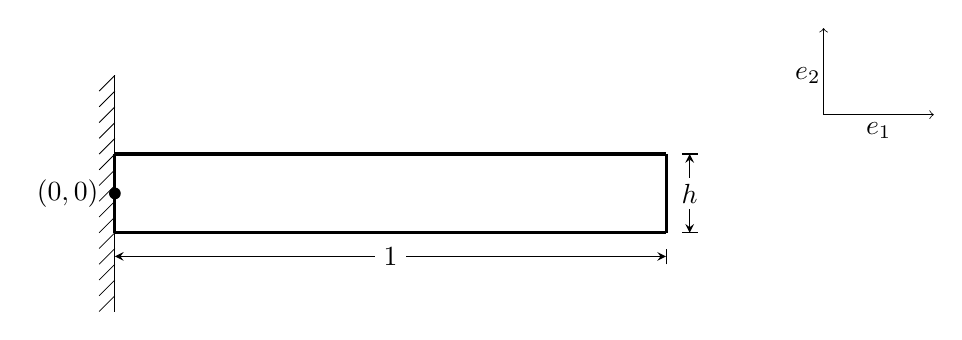
\begin{tikzpicture}
                    
                    \draw[line width = 0.4mm] (0,0.5) -- (7,0.5);
                    \draw[line width = 0.4mm] (0,-0.5) -- (7,-0.5);
                    \draw[line width = 0.4mm] (7,-0.5) -- (7,0.5);
                    \draw[line width = 0.4mm] (0,-0.5) -- (0,0.5);
                    
                    \draw[line width = 0.1mm] (0,1.5) -- (0,-1.5);
                    
                    \draw[line width = 0.1mm] (0,1.5) -- (-0.2,1.3);
                    \draw[line width = 0.1mm] (0,1.3) -- (-0.2,1.1);
                    \draw[line width = 0.1mm] (0,1.1) -- (-0.2,0.9);
                    \draw[line width = 0.1mm] (0,0.9) -- (-0.2,0.7);
                    \draw[line width = 0.1mm] (0,0.7) -- (-0.2,0.5);
                    \draw[line width = 0.1mm] (0,0.5) -- (-0.2,0.3);
                    \draw[line width = 0.1mm] (0,0.3) -- (-0.2,0.1);
                    \draw[line width = 0.1mm] (0,0.1) -- (-0.2,-0.1);
                    \draw[line width = 0.1mm] (0,-0.1) -- (-0.2,-0.3);
                    \draw[line width = 0.1mm] (0,-0.3) -- (-0.2,-0.5);
                    \draw[line width = 0.1mm] (0,-0.5) -- (-0.2,-0.7);
                    \draw[line width = 0.1mm] (0,-0.7) -- (-0.2,-0.9);
                    \draw[line width = 0.1mm] (0,-0.9) -- (-0.2,-1.1);
                    \draw[line width = 0.1mm] (0,-1.1) -- (-0.2,-1.3);
                    \draw[line width = 0.1mm] (0,-1.3) -- (-0.2,-1.5);
                    
                    \node at (7.3,0) {$h$};
                    \draw[-stealth] (7.3,0.2) -- (7.3,0.5);
                    \draw (7.2,0.5) -- (7.4,0.5);
                    \draw[-stealth] (7.3,-0.2) -- (7.3,-0.5);
                    \draw (7.2,-0.5) -- (7.4,-0.5);
                    
                    \node at (3.5,-0.8) {$1$};
                    \draw[stealth-] (0,-0.8) -- (3.3,-0.8);
                    \draw[stealth-] (7,-0.8) -- (3.7,-0.8);
                    \draw (7,-0.9) -- (7,-0.7);
                    
                    \draw[line width = 0.1mm,->] (9,1) -- (10.4,1);
                    \draw[line width = 0.1mm,->] (9,1) -- (9,2.1);
                    \node at (9.7,0.8) {$e_1$};
                    \node at (8.8,1.5) {$e_2$};
                    
                    \node at (-0.6,0) {$(0,0)$};
                    \node at (0,0)[circle,fill,inner sep=1.5pt]{};
                    
                \end{tikzpicture}
                \caption{A cantilever two-dimensional elastic body.}
            \end{figure} 
        
            % Placeholder for boundary conditions of 2D cantilever
            Boundary Conditions:
            \begin{eqnarray*}
                u & = & 0 \quad \textrm{ where } x_1 = 0\\
                Tn & = & 0 \quad \textrm{ on the rest of the body }
            \end{eqnarray*} With $n$ the outward normal vector to $\Omega$.
        \end{frame}

    \subsection{Three-dimensional cantilever beam}
        \begin{frame}{Models - Three-dimensional cantilever beam}
            \begin{columns}[T] % align columns
                \begin{column}{.6\textwidth}
                    \only<1->{ % Frame 1: Equations of motion
                        Equations of motion
                        \begin{eqnarray*}
                            \partial_t^2 u & = & \textrm{div}T + Q
                        \end{eqnarray*}
                        with
                        \begin{eqnarray*}
                            \textrm{div}  T & = &
                            \begin{bmatrix}
                                \partial_1 \sigma_{11} + \partial_2 \sigma_{12} + \partial_3 \sigma_{13} \\
                                \partial_1 \sigma_{21} + \partial_2 \sigma_{22} + \partial_3 \sigma_{23} \\
                                \partial_1 \sigma_{31} + \partial_2 \sigma_{32} + \partial_3 \sigma_{33}
                            \end{bmatrix}.\label{eq:3D_Model:divT-D}
                        \end{eqnarray*}
                    }
                    \only<1->{ % Frame 1: Constitutive equations
                        Constitutive equations
                        \begin{eqnarray*}
                            T = \frac{1}{\gamma(1+\nu)} \mathcal{E} + \frac{\nu}{\gamma(1+\nu)(1-2\nu)}\textrm{Tr}(\mathcal{E})I
                        \end{eqnarray*}
                    }
                \end{column}
                
                \begin{column}{.4\textwidth}
                    \only<2->{ % Frame 2: Parameter descriptions
                        \textbf{Description:}
                        \begin{itemize}
                            \item[-] \( u \): Displacement vector in 2D
                            \item[-] \( T \): Stress tensor
                            \item[-] \( Q \): External distributed load in 2D
                            \item[-] \( \mathcal{E} \): Young's modulus
                            \item[-] \( \nu \): Poisson's ratio
                            \item[-] \( \gamma \): Dimensionless constant
                        \end{itemize}
                    }
                \end{column}
            \end{columns}
        \end{frame}

        \begin{frame}{Models - Three-dimensional cantilever beam}
            \begin{figure}[h!]
                \centering
                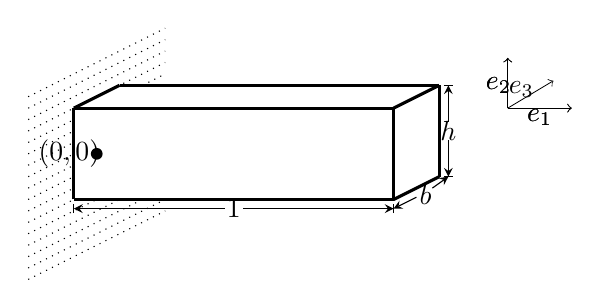
\begin{tikzpicture}[scale=0.58]
                    
                    \draw[line width = 0.4mm] (-0.5,1) -- (6.5,1);
                    \draw[line width = 0.4mm] (-0.5,-1) -- (6.5,-1);
                    \draw[line width = 0.4mm] (6.5,-1) -- (6.5,1);
                    \draw[line width = 0.4mm] (-0.5,-1) -- (-0.5,1);
                    
                    \draw[line width = 0.4mm] (0.5,1.5) -- (7.5,1.5);
                    \draw[line width = 0.4mm] (7.5,-0.5) -- (7.5,1.5);
                    
                    
                    \draw[line width = 0.4mm] (-0.5,1) -- (0.5,1.5);
                    \draw[line width = 0.4mm] (6.5,1) -- (7.5,1.5);
                    \draw[line width = 0.4mm] (6.5,-1) -- (7.5,-0.5);
                    
                    
                    
                    \draw[scale=0.5, domain=-3:3, smooth, variable=\x,dotted] plot ({\x}, {0.5*\x+4});
                    \draw[scale=0.5, domain=-3:3, smooth, variable=\x,dotted] plot ({\x}, {0.5*\x+3.5});
                    \draw[scale=0.5, domain=-3:3, smooth, variable=\x,dotted] plot ({\x}, {0.5*\x+3});
                    \draw[scale=0.5, domain=-3:3, smooth, variable=\x,dotted] plot ({\x}, {0.5*\x+2.5});
                    
                    \draw[scale=0.5, domain=-3:-1, smooth, variable=\x,dotted] plot ({\x}, {0.5*\x+2});
                    \draw[scale=0.5, domain=2:3, smooth, variable=\x,dotted] plot ({\x}, {0.5*\x+2});
                    
                    \draw[scale=0.5, domain=-3:-1, smooth, variable=\x,dotted] plot ({\x}, {0.5*\x+1.5});
                    \draw[scale=0.5, domain=-3:-1, smooth, variable=\x,dotted] plot ({\x}, {0.5*\x+1});
                    \draw[scale=0.5, domain=-3:-1, smooth, variable=\x,dotted] plot ({\x}, {0.5*\x+0.5});
                    \draw[scale=0.5, domain=-3:-1, smooth, variable=\x,dotted] plot ({\x}, {0.5*\x});
                    \draw[scale=0.5, domain=-3:-1, smooth, variable=\x,dotted] plot ({\x}, {0.5*\x-0.5});
                    \draw[scale=0.5, domain=-3:-1, smooth, variable=\x,dotted] plot ({\x}, {0.5*\x-1});
                    \draw[scale=0.5, domain=-3:-1, smooth, variable=\x,dotted] plot ({\x}, {0.5*\x-1.5});
                    \draw[scale=0.5, domain=-3:0, smooth, variable=\x,dotted] plot ({\x}, {0.5*\x-2});
                    \draw[scale=0.5, domain=-3:1, smooth, variable=\x,dotted] plot ({\x}, {0.5*\x-2.5});
                    \draw[scale=0.5, domain=-3:2, smooth, variable=\x,dotted] plot ({\x}, {0.5*\x-3});
                    \draw[scale=0.5, domain=-3:3, smooth, variable=\x,dotted] plot ({\x}, {0.5*\x-3.5});
                    \draw[scale=0.5, domain=-3:3, smooth, variable=\x,dotted] plot ({\x}, {0.5*\x-4});
                    
                    %\node at (6.9,1) {$b$};
                    %\node at (6.65,0) {$h$};
                    %\node at (3.2,-1.2) {$\ell = 1$};
                    
                    \draw[line width = 0.1mm,->] (9,1) -- (10,1.6);
                    \draw[line width = 0.1mm,->] (9,1) -- (10.4,1);
                    \draw[line width = 0.1mm,->] (9,1) -- (9,2.1);
                    \node at (9.3,1.4) {$e_3$};
                    \node at (9.7,0.8) {$e_1$};
                    \node at (8.8,1.5) {$e_2$};
                    
                    \node at (7.7,0.5) {$h$};
                    \draw[-stealth] (7.7,0.7) -- (7.7,1.5);
                    \draw (7.6,1.5) -- (7.8,1.5);
                    \draw[-stealth] (7.7,0.3) -- (7.7,-0.5);
                    \draw (7.6,-0.5) -- (7.8,-0.5);
                    
                    \node at (3,-1.2) {$1$};
                    \draw[stealth-] (-0.5,-1.2) -- (2.8,-1.2);
                    \draw[stealth-] (6.5,-1.2) -- (3.2,-1.2);
                    \draw (6.5,-1.3) -- (6.5,-1.1);
                    \draw (-0.5,-1.3) -- (-0.5,-1.1);
                    
                    \node at (7.2,-0.9) {$b$};
                    \draw[stealth-] (7.7,-0.5) -- (7.35,-0.75);
                    \draw[stealth-] (6.5,-1.2) -- (7,-0.95);
                    
                    \draw[line width = 0.1mm,->] (9,1) -- (10.4,1);
                    \draw[line width = 0.1mm,->] (9,1) -- (9,2.1);
                    \node at (9.7,0.8) {$e_1$};
                    \node at (8.8,1.5) {$e_2$};
                    
                    \node at (-0.6,0) {$(0,0)$};
                    \node at (0,0)[circle,fill,inner sep=1.5pt]{};
                    
                    %\node at (-1.4,-1.3) {$(0,-\frac{h}{2},-\frac{b}{2})$};
                    %\node at (-1.4,1) {$(0,\frac{h}{2},-\frac{b}{2})$};
                    %\node at (0.5,1.8) {$(0,\frac{h}{2},\frac{b}{2})$};
                    
                    %\node at (6,-1.3) {$(1,-\frac{h}{2},-\frac{b}{2})$};
                    %\node at (6.3,0.7) {$(1,\frac{h}{2},-\frac{b}{2})$};
                    %\node at (7.5,1.8) {$(1,\frac{h}{2},\frac{b}{2})$};
                    %\node at (8.4,-0.4) {$(1,-\frac{h}{2},\frac{b}{2})$};
                    
                \end{tikzpicture}
                \caption{Cantilever Three-Dimensional Elastic Body with Rectangular Cross-Section.}
            \end{figure} 
            Boundary Conditions:
            \begin{eqnarray*}
                u & = & 0 \quad \textrm{ where } x_1 = 0\\
                Tn & = & 0 \quad \textrm{ on the rest of the body }
            \end{eqnarray*} With $n$ the outward normal vector to $\Omega$.
        \end{frame}

\section{Literature study}
    \subsection{Comparison of linear beam theories}
        \begin{frame}{Literature study - Comparison of linear beam theories}
            Consider the article [\cite{LVV09}]\footfullcite{LVV09}
        \end{frame}

    \subsection{Empirical comparison of beams}
        \begin{frame}{Literature study - Empirical comparison of beams}
            Consider the article [\cite{SP06}]\footfullcite{SP06}
        \end{frame}

\section{Numerical Results}
    \subsection{Finite Element Analysis}
        \begin{frame}{Eigenvalue problem - Two and Three-dimensional models}
            General eigenvalue problem for the two- and three-dimensional models:
            
                For the eigenvalue problem, assume that $M_{f}Q^I = 0$ so that 
            \begin{eqnarray}
                    M\ddot{\bar{u}} & = & K\bar{u}.\label{eq:2DFEM:M2}
            \end{eqnarray}
            
            Not so simple to compute the eigenvalues and eigenfunctions.
            
            Need to use a numerical method like FEM to approximate the eigenvalues and eigenvectors.
        
        \end{frame}
        
        \begin{frame}{Eigenvalue problem - Timoshenko model}
            General eigenvalue problem for the Timoshenko beam model:
        
            Find functions $u$ and $\phi$ and a real number $\lambda$ satisfying the following equations
            \begin{eqnarray}
            -u'' + \phi' &=& \lambda u, \label{eq:Timo:EigenvalueProblem1}\\
            -\alpha u' + \alpha\phi - \frac{1}{\gamma}\phi'' &=& \lambda\phi.\label{eq:Timo:EigenvalueProblem2}
            \end{eqnarray}
        
            The solution to this problem is presented in the article [\cite{VV06}]\footfullcite{VV06}.
        
            \begin{itemize}
                \item[-] Provides a method to calculate the exact eigenvalues.
                \item[-] Uses a cantilever beam as an example in the article.
                \item[-] Eigenvalues can be numerically obtained to any degree of accuracy.
            \end{itemize}
        
        \end{frame}

        \begin{frame}{FEM}
        \end{frame}

        \begin{frame}{Accuracy of the Eigenvalues}
            \centering
            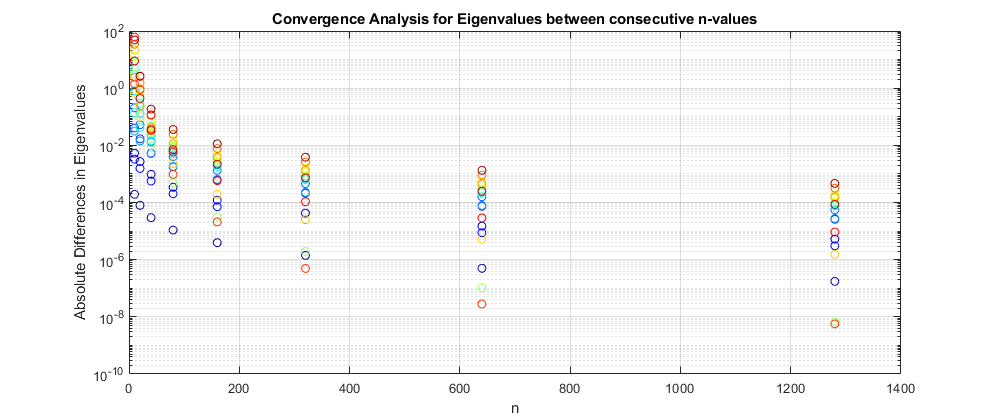
\includegraphics[scale=0.3]{Convergence.png} \\ % Adjust scale as needed
            \footnotesize Rate of convergence of the first 20 eigenvalues.

            \centering
            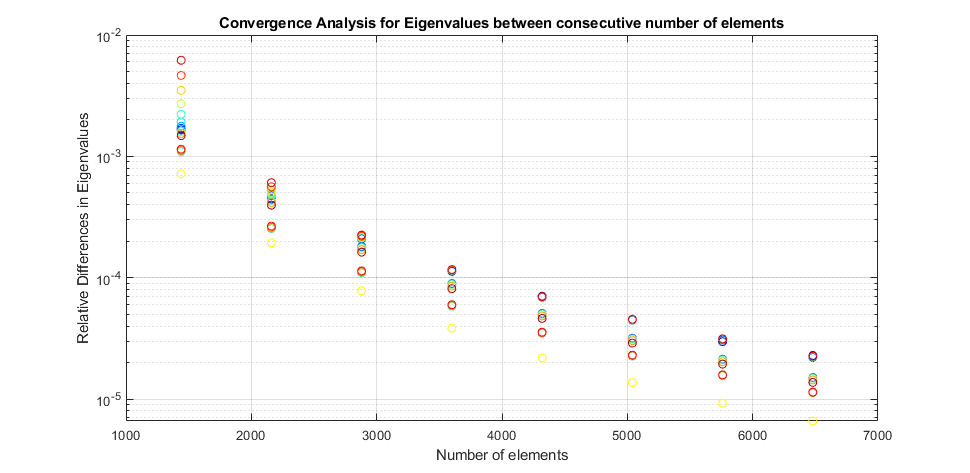
\includegraphics[scale=0.3]{convergence3d.png} \\ % Adjust scale as needed
            \footnotesize Rate of convergence of the first 20 eigenvalues.
        \end{frame}

    \subsection{Validity of the Timoshenko beam model}
        \begin{frame}{Validity of the Timoshenko beam model}
            \begin{center}
                \begin{minipage}[b]{0.45\linewidth}
                    \centering
                    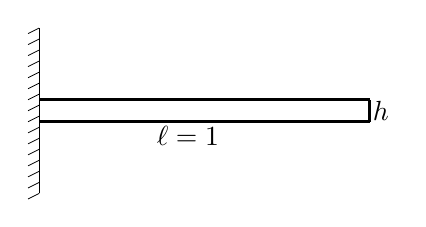
\begin{tikzpicture}[scale=0.7]
                        \draw[line width = 0.4mm] (0,0.2) -- (6,0.2);
                                    \draw[line width = 0.4mm] (0,-0.2) -- (6,-0.2);
                                    \draw[line width = 0.4mm] (6,-0.2) -- (6,0.2);
                                    
                                    \node at (6.2,0) {$h$};
                                    \node at (2.7,-0.45) {$\ell = 1$};
                                    
                                    \draw[line width = 0.1mm] (0,-1.5) -- (0,1.5);
                                    \draw[line width = 0.1mm] (0,1.5) -- (-0.2,1.4);
                                    \draw[line width = 0.1mm] (0,1.3) -- (-0.2,1.2);
                                    \draw[line width = 0.1mm] (0,1.1) -- (-0.2,1);
                                    \draw[line width = 0.1mm] (0,0.9) -- (-0.2,0.8);
                                    \draw[line width = 0.1mm] (0,0.7) -- (-0.2,0.6);
                                    \draw[line width = 0.1mm] (0,0.5) -- (-0.2,0.4);
                                    \draw[line width = 0.1mm] (0,0.3) -- (-0.2,0.2);
                                    \draw[line width = 0.1mm] (0,0.1) -- (-0.2,0);
                                    
                                    \draw[line width = 0.1mm] (0,-0.1) -- (-0.2,-0.2);
                                    \draw[line width = 0.1mm] (0,-0.3) -- (-0.2,-0.4);
                                    \draw[line width = 0.1mm] (0,-0.5) -- (-0.2,-0.6);
                                    \draw[line width = 0.1mm] (0,-0.7) -- (-0.2,-0.8);
                                    \draw[line width = 0.1mm] (0,-0.9) -- (-0.2,-1);
                                    \draw[line width = 0.1mm] (0,-1.1) -- (-0.2,-1.2);
                                    \draw[line width = 0.1mm] (0,-1.3) -- (-0.2,-1.4);
                                    \draw[line width = 0.1mm] (0,-1.5) -- (-0.2,-1.6);
                    \end{tikzpicture}
                    \captionof{figure}{Two-Dimensional Beam}
                \end{minipage}
                \hfill
                \begin{minipage}[b]{0.45\linewidth}
                    \centering
                    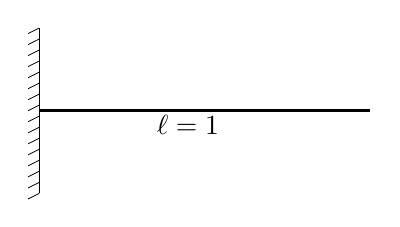
\begin{tikzpicture}[scale=0.7]
                        \draw[line width = 0.4mm] (0,0) -- (6,0);
                                \node at (2.7,-0.25) {$\ell = 1$};
                                
                                \draw[line width = 0.1mm] (0,-1.5) -- (0,1.5);
                                \draw[line width = 0.1mm] (0,1.5) -- (-0.2,1.4);
                                \draw[line width = 0.1mm] (0,1.3) -- (-0.2,1.2);
                                \draw[line width = 0.1mm] (0,1.1) -- (-0.2,1);
                                \draw[line width = 0.1mm] (0,0.9) -- (-0.2,0.8);
                                \draw[line width = 0.1mm] (0,0.7) -- (-0.2,0.6);
                                \draw[line width = 0.1mm] (0,0.5) -- (-0.2,0.4);
                                \draw[line width = 0.1mm] (0,0.3) -- (-0.2,0.2);
                                \draw[line width = 0.1mm] (0,0.1) -- (-0.2,0);
                                
                                \draw[line width = 0.1mm] (0,-0.1) -- (-0.2,-0.2);
                                \draw[line width = 0.1mm] (0,-0.3) -- (-0.2,-0.4);
                                \draw[line width = 0.1mm] (0,-0.5) -- (-0.2,-0.6);
                                \draw[line width = 0.1mm] (0,-0.7) -- (-0.2,-0.8);
                                \draw[line width = 0.1mm] (0,-0.9) -- (-0.2,-1);
                                \draw[line width = 0.1mm] (0,-1.1) -- (-0.2,-1.2);
                                \draw[line width = 0.1mm] (0,-1.3) -- (-0.2,-1.4);
                                \draw[line width = 0.1mm] (0,-1.5) -- (-0.2,-1.6);
                    \end{tikzpicture}
                    \captionof{figure}{Timoshenko Beam}
                \end{minipage}
            \end{center}
        \end{frame}
        
        \begin{frame}{Comparison of two and three-dimensional models}
            \centering
            \begin{minipage}[b]{0.45\textwidth}
                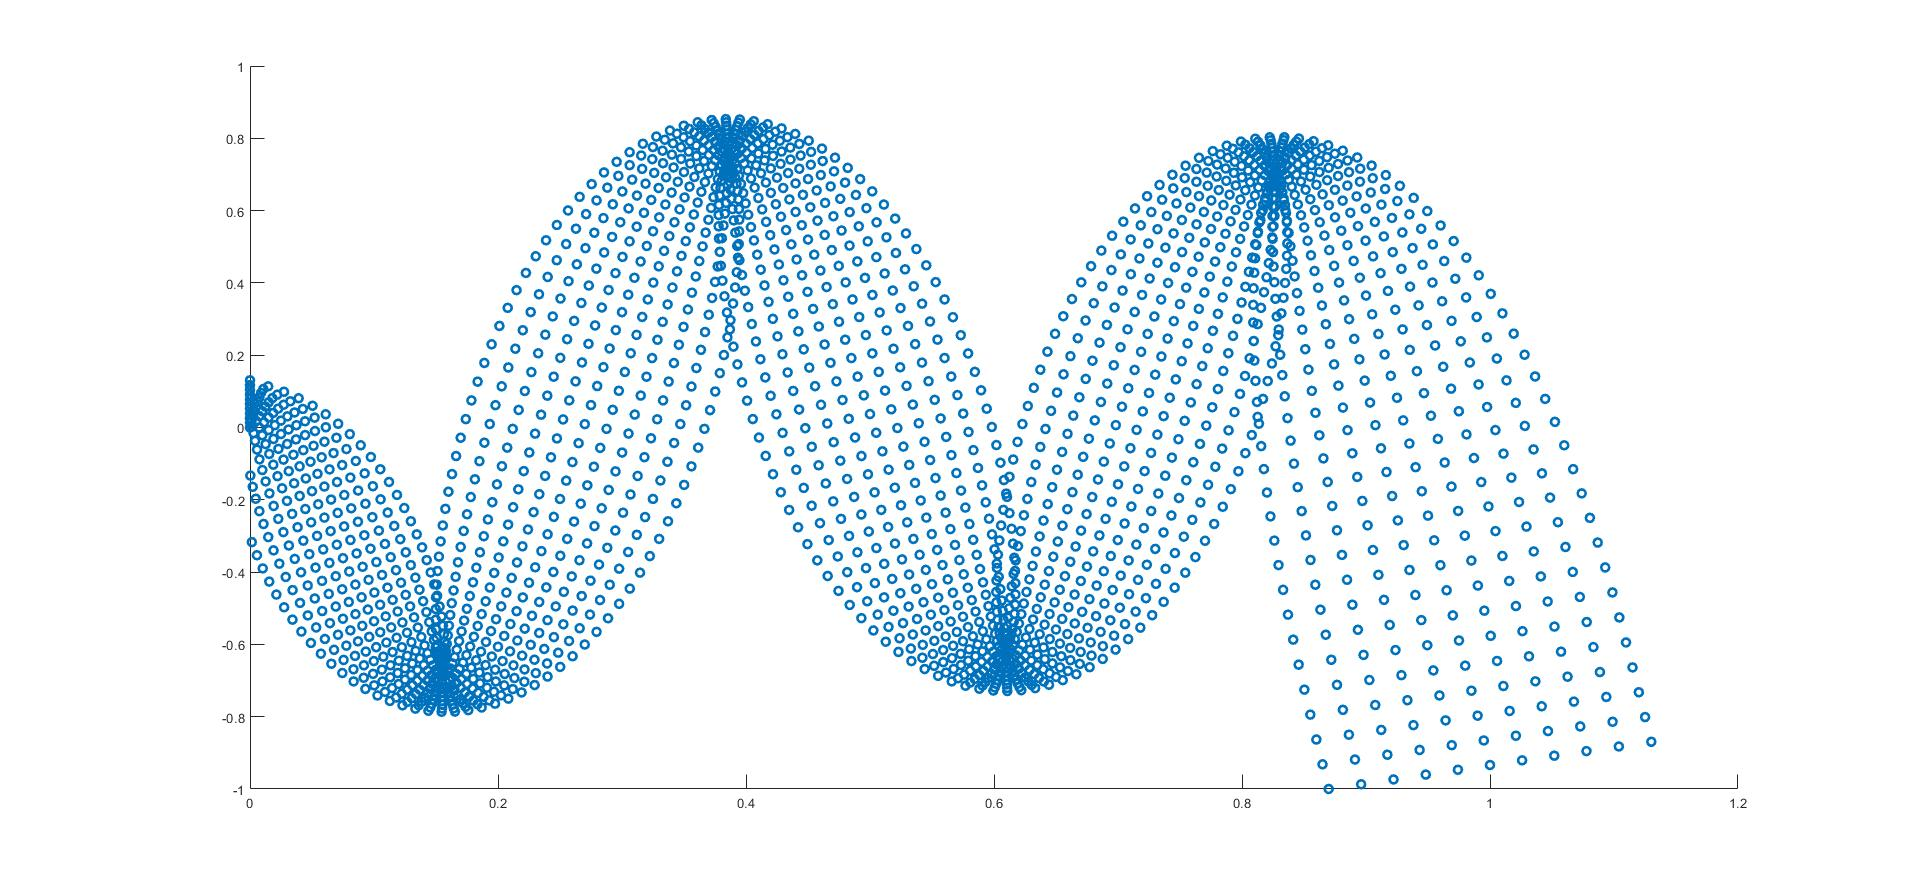
\includegraphics[width=\textwidth]{Beam1.jpg}
                \\ 2D Beam Type - $\lambda_6 = 21.911$
                \label{fig:minipage2}
            \end{minipage}
            \hfill
            \begin{minipage}[b]{0.45\textwidth}
                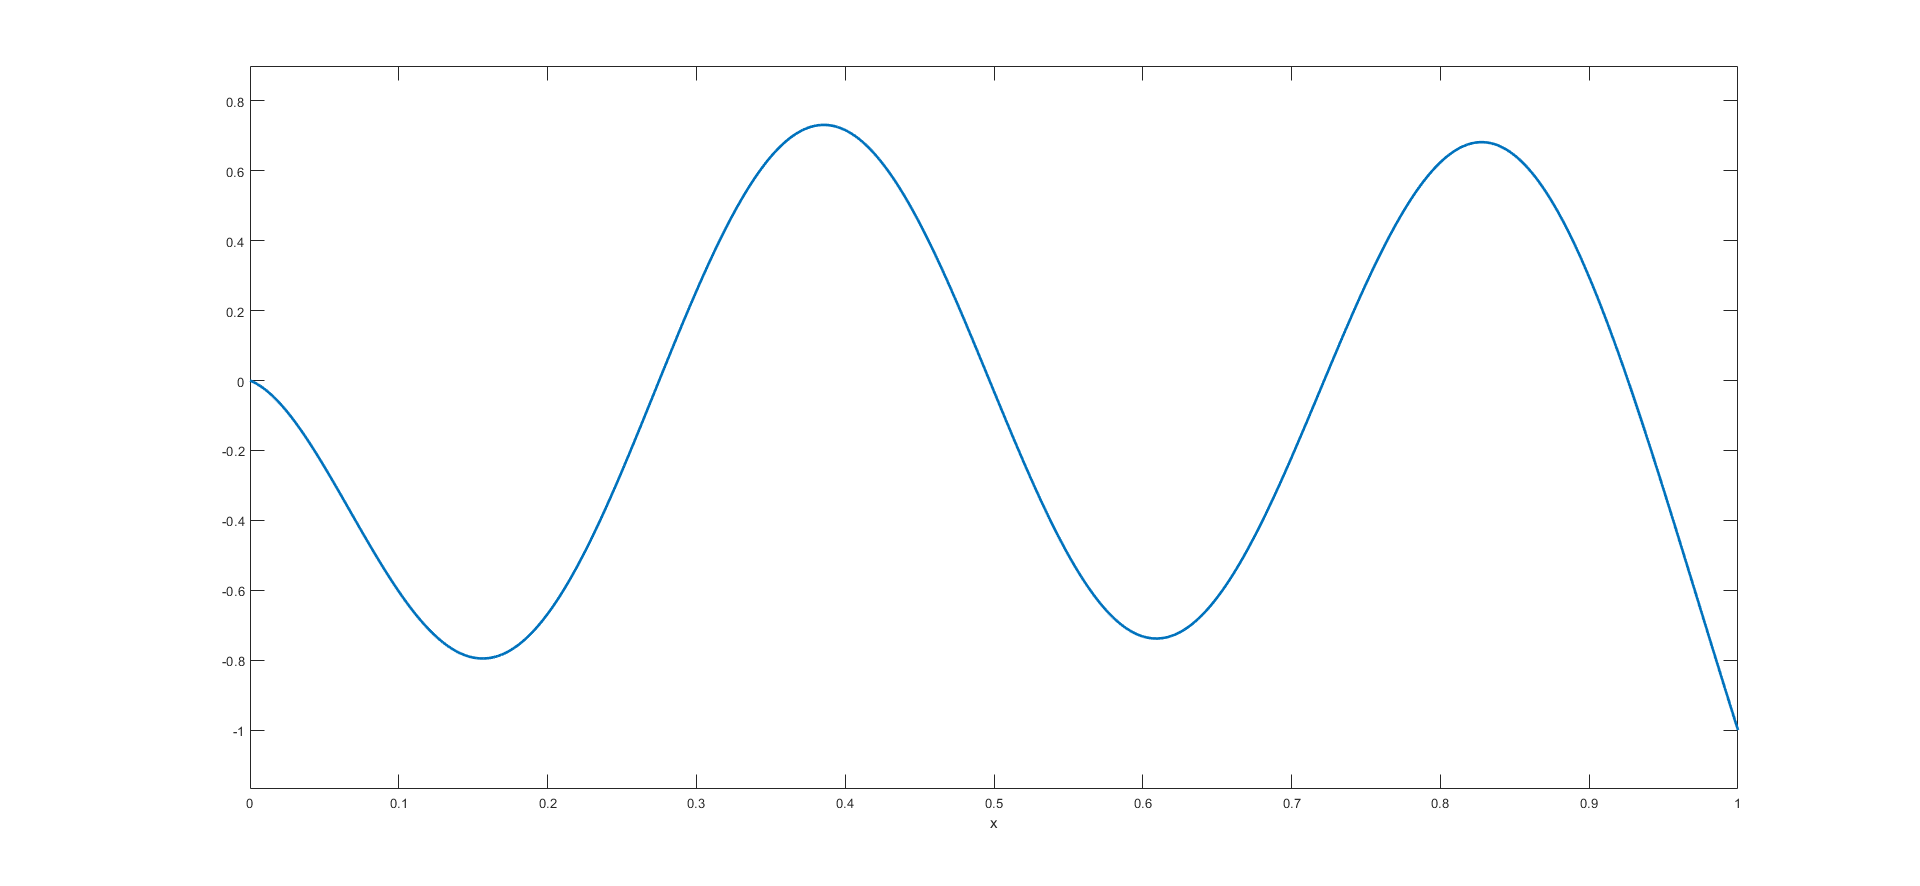
\includegraphics[width=\textwidth]{1DBeam2.png}
                \\ Timoshenko - $\lambda_5 = 21.794$
                \label{fig:minipage1}
            \end{minipage}
            \vspace{1em}
            \begin{minipage}[b]{0.45\textwidth}
                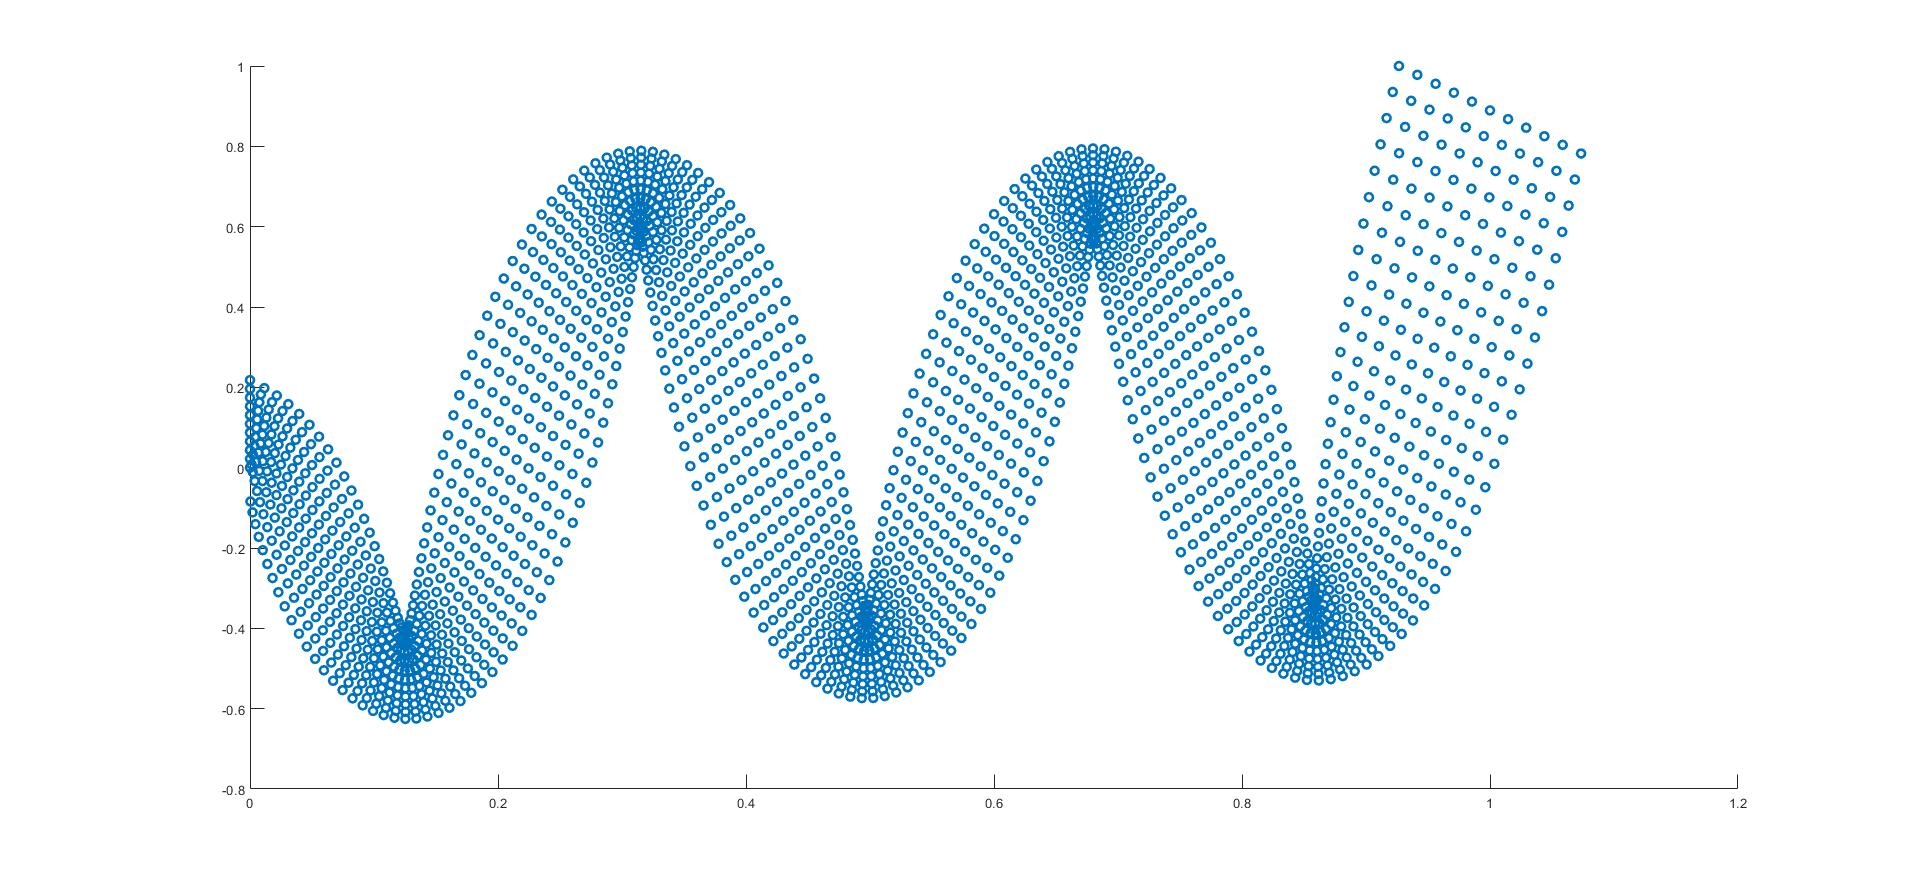
\includegraphics[width=\textwidth]{Beam2.jpg}
                \\ 2D Beam Type - $\lambda_7 = 45.711$
                \label{fig:minipage4}
            \end{minipage}
            \hfill
            \begin{minipage}[b]{0.45\textwidth}
                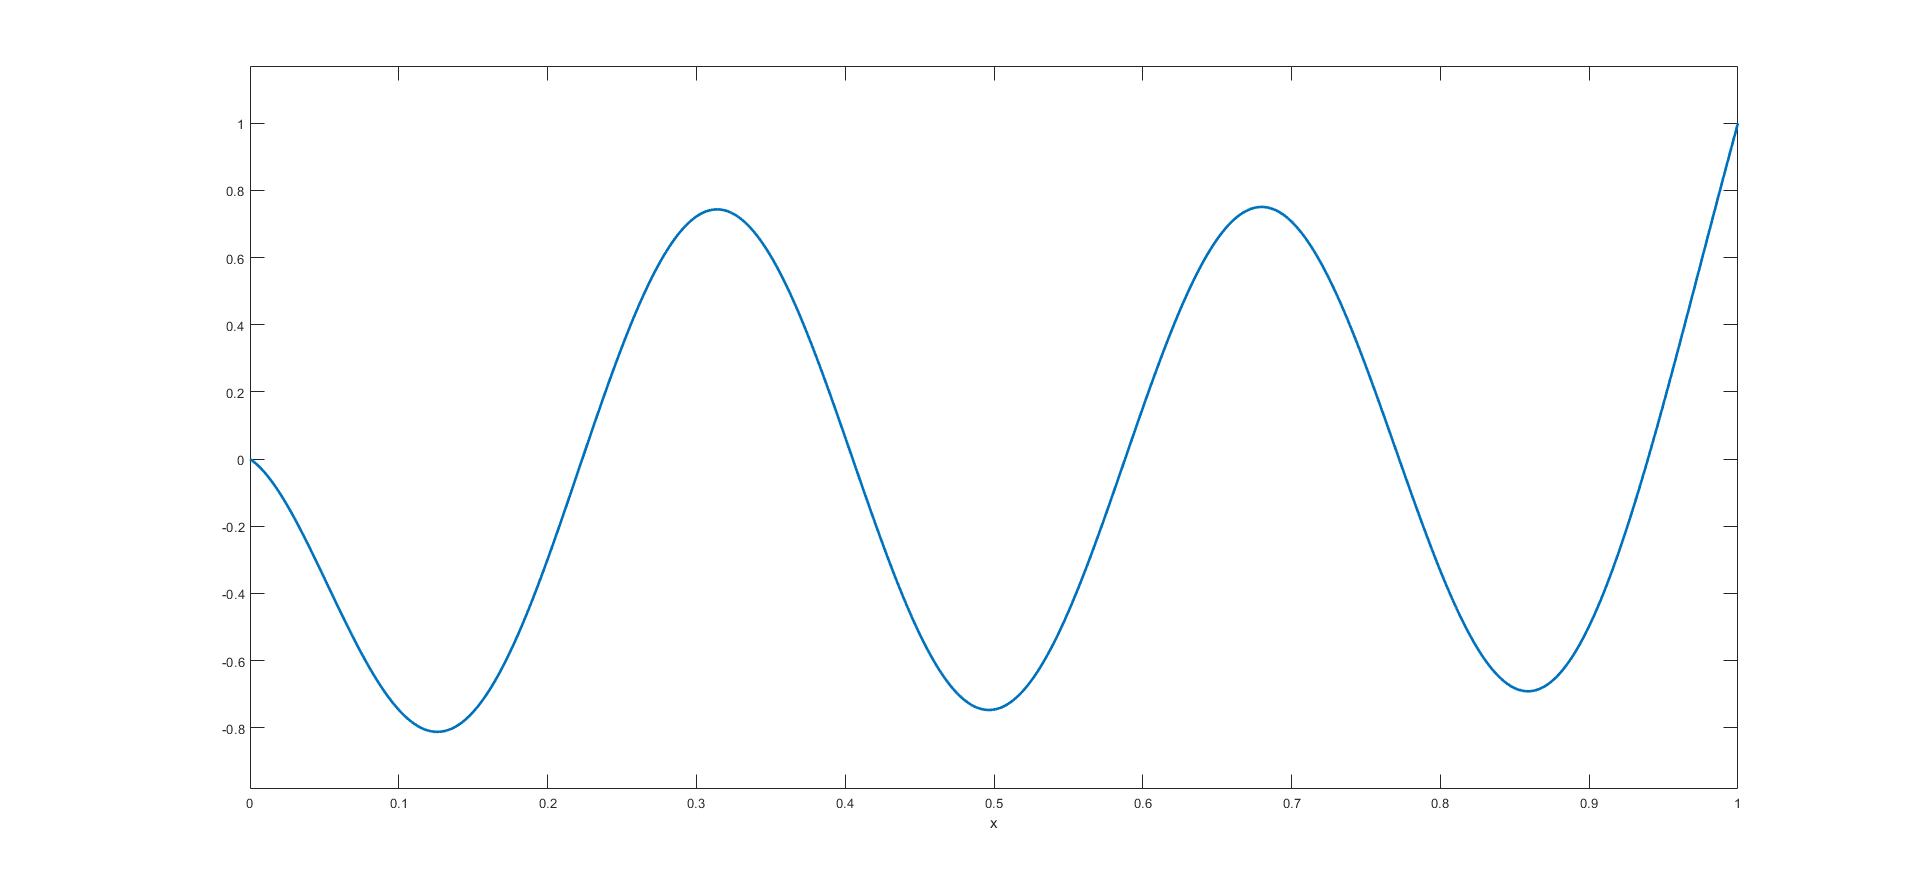
\includegraphics[width=\textwidth]{1DBeam1.png}
                \\ Timoshenko - $\lambda_6 = 45.390$
                \label{fig:minipage3}
            \end{minipage}
            \\ Modal shapes of the displacement $w$ for the beam-type 2D body and the Timoshenko beam with $\alpha = 4800$ ($h = 1/20$).
        \end{frame}
        
        
        \begin{frame}{Comparison of two and three-dimensional models}
            \centering
            \begin{minipage}[b]{0.45\textwidth}
                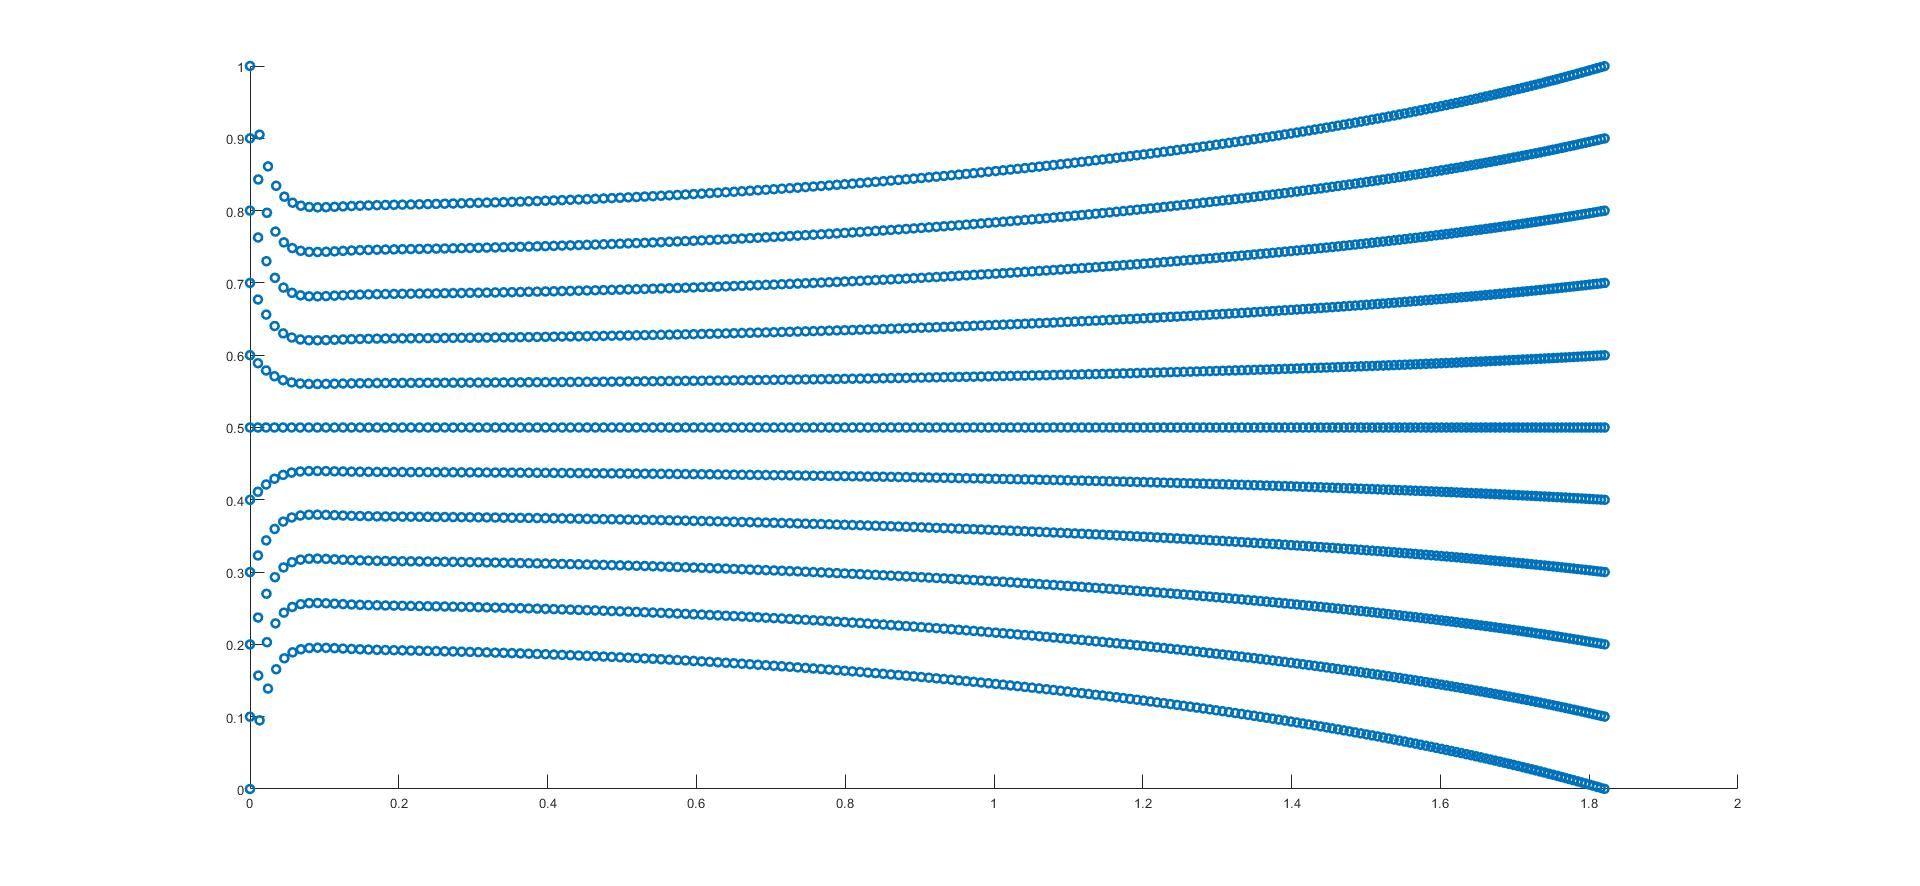
\includegraphics[width=\textwidth]{NotBeam1.jpg}
                \\ Non-Beam Type - $\lambda_4 = 7.7077$
                \label{fig:nonbeam1}
            \end{minipage}
            \hfill
            \begin{minipage}[b]{0.45\textwidth}
                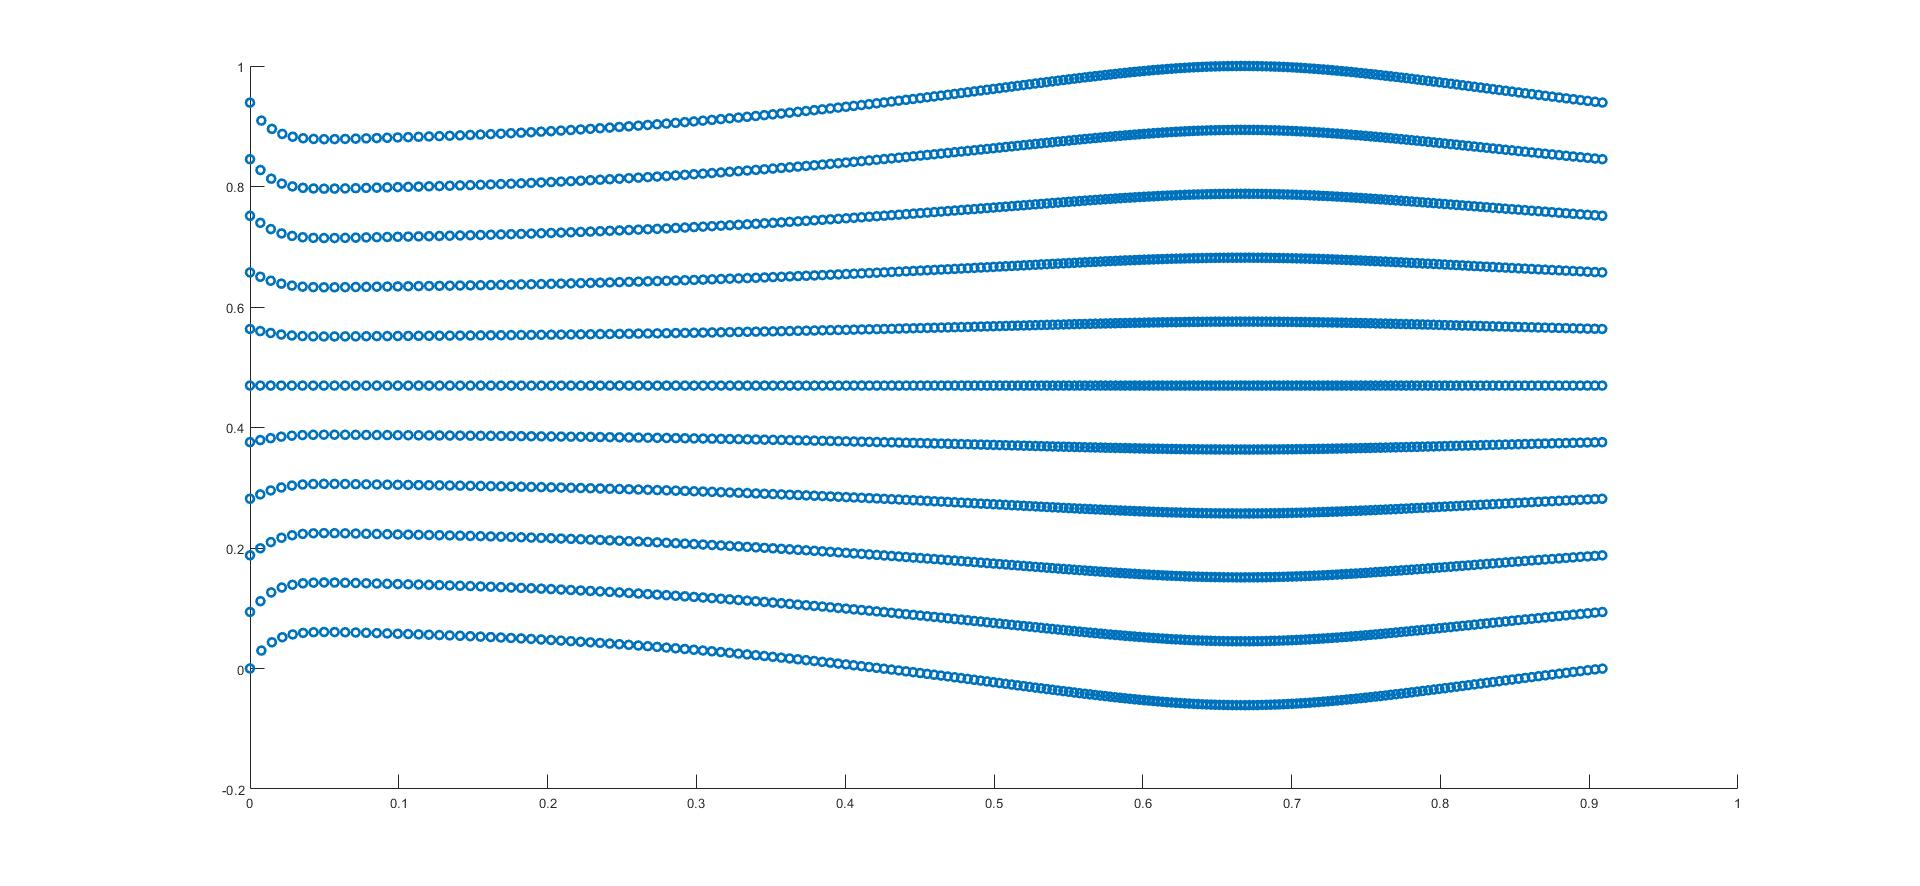
\includegraphics[width=\textwidth]{NotBeam2.jpg}
                \\ Non-Beam Type - $\lambda_8 = 69.344$
                \label{fig:nonbeam2}
            \end{minipage}
            \\ Modal shapes of the displacement $w$ for the non-beam type 2D body with $h = 1/20$.
        \end{frame}
        
        
        \begin{frame}{Comparison of two and three-dimensional models}
            \centering
            \footnotesize
            \renewcommand{\arraystretch}{0.9}
            Results from [LVV09] and results obtained. $0^a$ indicates a 0 due to rounding. $\alpha = 1200$
        
            \begin{tabular}{cccc|cccc}
                \hline
                & \multicolumn{3}{c}{[LVV09]} & & \multicolumn{3}{c}{Dissertation} \\
                
                & 2D & Timo & RE & & 2D & Timo & RE \\
                \hline
                1 & 0.0317 & 0.0316 & 0.00315 & 1 & 0.031713 & 0.031639 & 0.0023407 \\
                2 & 1.14 & 1.14 & $0^a$ & 2 & 1.1413 & 1.1365 & 0.0042050 \\
                3 & 7.72 & - & - & 3 & 7.7161 & - & - \\
                4 & 7.92 & 7.86 & 0.00758 & 4 & 7.918 & 7.8617 & 0.0071116 \\
                5 & 26.2 & 25.9 & 0.0115 & 5 & 26.148 & 25.869 & 0.010669 \\
                6 & 60.8 & 59.9 & 0.0148 & 6 & 60.816 & 59.946 & 0.014303 \\
                7 & 69.3 & - & - & 7 & 69.344 & - & - \\
                8 & 115 & 113 & 0.0174 & 8 & 115.28 & 113.23 & 0.017787 \\
                9 & 192 & 188 & 0.0208 & 9 & 191.57 & 187.55 & 0.020999 \\
                10 & 192 & - & - & 10 & 192.03 & - & - \\
                11 & 291 & 284 & 0.0241 & 11 & 290.76 & 283.81 & 0.023899 \\
                \hline
            \end{tabular}
        
        \end{frame}
        
        \begin{frame}{Eigenvalue problem - FEM}
            \centering
            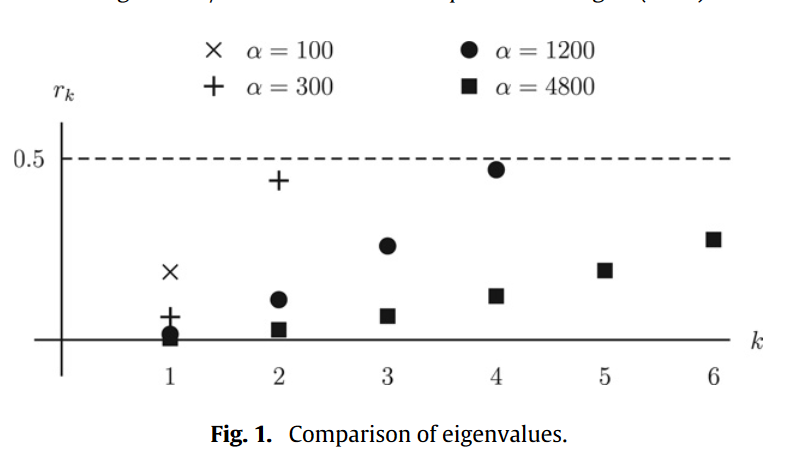
\includegraphics[scale=0.45]{Result.png} \\ % Adjust scale as needed
            \footnotesize Rate of convergence of the first 20 eigenvalues.
            \label{fig:conv}
        \end{frame}
        
        \begin{frame}{Comparison of Eigenvalues across Different Parameters}
            \centering
            \footnotesize
            \renewcommand{\arraystretch}{0.8}
            \resizebox{\textwidth}{!}{%
            \begin{tabular}{|cccc||cccc||cccc||cccc|}
                \hline
                \multicolumn{16}{|c|}{Comparison of Eigenvalues} \\
                \hline\hline
                \multicolumn{4}{|c||}{ $h = 1/5$ or $\alpha = 300$} & \multicolumn{4}{c||}{$h =1/10$ or $\alpha = 1200$} & \multicolumn{4}{c||}{$h = 1/20$ or $\alpha = 4800$} & \multicolumn{4}{c|}{$h = 1/30$ or $\alpha = 10800$} \\
                \hline
        
                {i} & {2D} & {j} & {Timo} & {i} & {2D} & {j} & {Timo} & {i} & {2D} & {j} & {Timo} & {i} & {2D} & {j} & {Timo} \\
                \hline
                {1}&0.12151&1&0.12092&1&0.031713&1&0.031639&1&0.008013&1&0.008004&1&0.003568&1&0.003565\\
                {2}&3.5460&2&3.5071&2&1.1413&2     & 1.1365 & 2     & 0.30756 & 2     & 0.30705 & 2     & 0.13869 & 2     & 0.13855 \\
                {3} & {7.7311} &       & {-} & {3}     & {7.7161} &       & {-} & 3     & 2.3273 & 3     & 2.3213 & 3     & 1.0698 & 3     & 1.0683 \\
                {4} & 20.225 & 3     & 19.869 & 4     & 7.9180 & 3     & 7.8617 & {4}     & {7.7077} &       & {-} & 4     & 4.0140 & 4     & 4.0058 \\
                {5} & 56.109 & 4     & 54.766 & 5     & 26.148 & 4     & 25.869 & 5     & 8.5086 & 4     & 8.4762 & {5}     & {7.7047} &       & {-} \\
                {6} & {69.164} &       & {-} & 6     & 60.816 & 5     & 59.946 & 6     & 21.911 & 5     & 21.794 & 6     & 10.655 & 5     & 10.625 \\
                {7} & 114.03 & 5     & 110.75 & {7}     & {69.344} &       & {-} & 7     & 45.711 & 6     & 45.390 & 7     & 22.975 & 6     & 22.890 \\
                {8} & {189.17} &  6     & {186.50} & 8     & 115.28 & 6     & 113.23 & {8}     & {69.344} &       & {-} & 8     & 43.113 & 7     & 42.909 \\
                {9} & {192.61} &      &  & {9}     & {191.57} &   7  & {187.55} & 9     & 82.887 & 7     & 82.154 & {9}     & {69.331} &       & {-} \\
                {10} & 285.85 & 7     & 277.64 & {10}    & {192.03} &      & {-} & 10    & 136.03 & 8     & 134.58 & 10    & 73.230 & 8     & 72.803 \\
                {11} & 328.40 & 8     & 330.29 & 11    & 290.76 & 8     & 283.81 & {11}    & {192.48} &       & {-} & 11    & 115.41 & 9     & 114.61 \\
                {12} & {357.08} &       & {-} & {12}    & {374.45} &       & {-} & 12    & 207.29 & 9     & 204.69 & 12    & 171.61 & 10    & 170.20 \\
                {13} & 397.33 & 9     & 394.02 & 13    & 413.20 & 9     & 402.27 & 13    & 298.38 & 10    & 294.10 & {13}    & {192.52} &       & {-} \\
                {14} & 442.00   & 10    & 439.52 & 14    & 558.67 & 10    & 542.65 & {14}    & {376.83} &       & {-} & 14    & 243.56 & 11    & 241.26 \\
                {15} & {533.71} &       & {-} & {15}    & {614.11} &       & {-} & 15    & 410.63 & 11    & 404.01 & 15    & 332.83 & 12    & 329.28 \\
                {16} & 538.97 & 11    & 541.55 & 16    & 726.26 & 11    & 704.15 & 16    & 545.03 & 12    & 535.32 & {16}    & {377.16} &       & {-} \\
                {17} & {596.06} &       & {-} & {17}    & {906.28} &       & {-} & {17}    & {621.95} &       & {-} & 17    & 440.77 & 13    & 435.51 \\
                {18} & 602.77 & 12    & 596.09 & 18    & 913.69 & 12    & 884.92 & 18    & 702.30 & 13    & 688.64 & 18    & 568.51 & 14    & 561.04 \\
                {19} & {657.87} &       & {-} & 19    & 1113.7 & 13    & 1080.1 & 19    & 882.95 & 14    & 864.40 & {19}    & {623.05} &       & {-} \\
                {20} & 717.37 & 13    & 731.74 & {20}    & {1218.0}  &       & {-} & {20}    & {927.18} &       & {-} & 20    & 717.04 & 15    & 706.74 \\
                \hline
                \multicolumn{2}{|c}{Max RE:} & \multicolumn{2}{c||}{3.1718\%} & \multicolumn{2}{c}{Max RE:} & \multicolumn{2}{c||}{3.1486\%} & \multicolumn{2}{c}{Max RE:} & \multicolumn{2}{c||}{2.1018\%} & \multicolumn{2}{c}{Max RE:} & \multicolumn{2}{c|}{1.4361\%} \\
                \hline
            \end{tabular}}
        \end{frame}
        
        
        
    
    \subsection{Validity of the Two-dimensional beam model}
        \begin{frame}{Validity of the Two-dimensional beam model}
            \begin{center}
                \begin{minipage}[b]{0.45\linewidth}
                    \centering
                    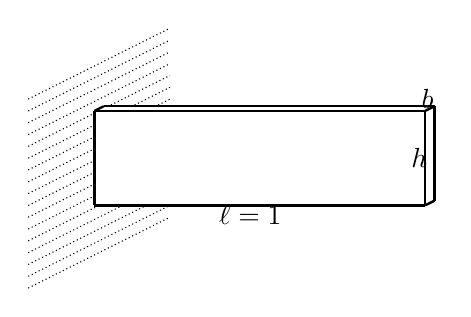
\begin{tikzpicture}[scale=0.6]
                        \draw[line width = 0.3mm] (-0.1,1) -- (6.9,1);
                        \draw[line width = 0.3mm] (-0.1,-1) -- (6.9,-1);
                        \draw[line width = 0.3mm] (6.9,-1) -- (6.9,1);
                        \draw[line width = 0.3mm] (-0.1,-1) -- (-0.1,1);
                        
                        \draw[line width = 0.3mm] (0.1,1.1) -- (7.1,1.1);
                        \draw[line width = 0.3mm] (7.1,-0.9) -- (7.1,1.1);
                        
                        \draw[line width = 0.3mm] (-0.1,1) -- (0.1,1.1);
                        \draw[line width = 0.3mm] (6.9,1) -- (7.1,1.1);
                        \draw[line width = 0.3mm] (6.9,-1) -- (7.1,-0.9);
                        
                        
                        
                        \draw[scale=0.5, domain=-3:3, smooth, variable=\x,densely dotted] plot ({\x}, {0.5*\x+4});
                        \draw[scale=0.5, domain=-3:3, smooth, variable=\x,densely dotted] plot ({\x}, {0.5*\x+3.5});
                        \draw[scale=0.5, domain=-3:3, smooth, variable=\x,densely dotted] plot ({\x}, {0.5*\x+3});
                        \draw[scale=0.5, domain=-3:3, smooth, variable=\x,densely dotted] plot ({\x}, {0.5*\x+2.5});
                        
                        \draw[scale=0.5, domain=-3:-0.1, smooth, variable=\x,densely dotted] plot ({\x}, {0.5*\x+2});
                        \draw[scale=0.5, domain=-3:-0.1, smooth, variable=\x,densely dotted] plot ({\x}, {0.5*\x+1.5});
                        \draw[scale=0.5, domain=-3:-0.1, smooth, variable=\x,densely dotted] plot ({\x}, {0.5*\x+1});
                        
                        \draw[scale=0.5, domain=0.5:3, smooth, variable=\x,densely dotted] plot ({\x}, {0.5*\x+2});
                        \draw[scale=0.5, domain=1.5:3, smooth, variable=\x,densely dotted] plot ({\x}, {0.5*\x+1.5});
                        \draw[scale=0.5, domain=2.5:3, smooth, variable=\x,densely dotted] plot ({\x}, {0.5*\x+1});
                        
                        \draw[scale=0.5, domain=-3:-0.1, smooth, variable=\x,densely dotted] plot ({\x}, {0.5*\x+0.5});
                        \draw[scale=0.5, domain=-3:-0.1, smooth, variable=\x,densely dotted] plot ({\x}, {0.5*\x});
                        \draw[scale=0.5, domain=-3:-0.1, smooth, variable=\x,densely dotted] plot ({\x}, {0.5*\x-0.5});
                        \draw[scale=0.5, domain=-3:-0.1, smooth, variable=\x,densely dotted] plot ({\x}, {0.5*\x-1});
                        \draw[scale=0.5, domain=-3:-0.1, smooth, variable=\x,densely dotted] plot ({\x}, {0.5*\x-1.5});
                        \draw[scale=0.5, domain=-3:0, smooth, variable=\x,densely dotted] plot ({\x}, {0.5*\x-2});
                        \draw[scale=0.5, domain=-3:1, smooth, variable=\x,densely dotted] plot ({\x}, {0.5*\x-2.5});
                        \draw[scale=0.5, domain=-3:2, smooth, variable=\x,densely dotted] plot ({\x}, {0.5*\x-3});
                        \draw[scale=0.5, domain=-3:3, smooth, variable=\x,densely dotted] plot ({\x}, {0.5*\x-3.5});
                        \draw[scale=0.5, domain=-3:3, smooth, variable=\x,densely dotted] plot ({\x}, {0.5*\x-4});
                        
                        \node at (6.95,1.25) {$b$};
                        \node at (6.78,0) {$h$};
                        \node at (3.2,-1.2) {$\ell = 1$};
                    \end{tikzpicture}
                    \captionof{figure}{Three-Dimensional Beam}
                \end{minipage}
                \hfill
                \begin{minipage}[b]{0.45\linewidth}
                    \centering
                    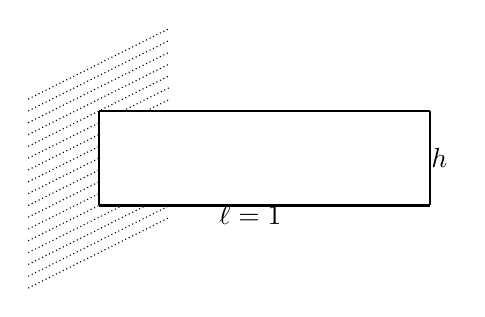
\begin{tikzpicture}[scale=0.6]
                        \draw[line width = 0.3mm] (0,1) -- (7,1);
                        \draw[line width = 0.3mm] (0,-1) -- (7,-1);
                        \draw[line width = 0.3mm] (7,-1) -- (7,1);
                        \draw[line width = 0.3mm] (0,-1) -- (0,1);
                        
                        
                        \draw[scale=0.5, domain=-3:3, smooth, variable=\x,densely dotted] plot ({\x}, {0.5*\x+4});
                        \draw[scale=0.5, domain=-3:3, smooth, variable=\x,densely dotted] plot ({\x}, {0.5*\x+3.5});
                        \draw[scale=0.5, domain=-3:3, smooth, variable=\x,densely dotted] plot ({\x}, {0.5*\x+3});
                        \draw[scale=0.5, domain=-3:3, smooth, variable=\x,densely dotted] plot ({\x}, {0.5*\x+2.5});
                        \draw[scale=0.5, domain=-3:3, smooth, variable=\x,densely dotted] plot ({\x}, {0.5*\x+2});
                        
                        \draw[scale=0.5, domain=-3:0, smooth, variable=\x,densely dotted] plot ({\x}, {0.5*\x+1.5});
                        \draw[scale=0.5, domain=-3:0, smooth, variable=\x,densely dotted] plot ({\x}, {0.5*\x+1});
                        
                        
                        \draw[scale=0.5, domain=1:3, smooth, variable=\x,densely dotted] plot ({\x}, {0.5*\x+1.5});
                        \draw[scale=0.5, domain=2:3, smooth, variable=\x,densely dotted] plot ({\x}, {0.5*\x+1});
                        
                        \draw[scale=0.5, domain=-3:0, smooth, variable=\x,densely dotted] plot ({\x}, {0.5*\x+0.5});
                        \draw[scale=0.5, domain=-3:0, smooth, variable=\x,densely dotted] plot ({\x}, {0.5*\x});
                        \draw[scale=0.5, domain=-3:0, smooth, variable=\x,densely dotted] plot ({\x}, {0.5*\x-0.5});
                        \draw[scale=0.5, domain=-3:0, smooth, variable=\x,densely dotted] plot ({\x}, {0.5*\x-1});
                        \draw[scale=0.5, domain=-3:0, smooth, variable=\x,densely dotted] plot ({\x}, {0.5*\x-1.5});
                        \draw[scale=0.5, domain=-3:0, smooth, variable=\x,densely dotted] plot ({\x}, {0.5*\x-2});
                        \draw[scale=0.5, domain=-3:1, smooth, variable=\x,densely dotted] plot ({\x}, {0.5*\x-2.5});
                        \draw[scale=0.5, domain=-3:2, smooth, variable=\x,densely dotted] plot ({\x}, {0.5*\x-3});
                        \draw[scale=0.5, domain=-3:3, smooth, variable=\x,densely dotted] plot ({\x}, {0.5*\x-3.5});
                        \draw[scale=0.5, domain=-3:3, smooth, variable=\x,densely dotted] plot ({\x}, {0.5*\x-4});
                        
                        \node at (7.2,0) {$h$};
                        \node at (3.2,-1.2) {$\ell = 1$};
                    \end{tikzpicture}
                    \captionof{figure}{Two-dimensional Beam}
                \end{minipage}
            \end{center}
        \end{frame}

        \begin{frame}{Three-Dimensional model vs Two-Dimensional model}
            \centering
            \begin{minipage}[b]{0.45\textwidth}
                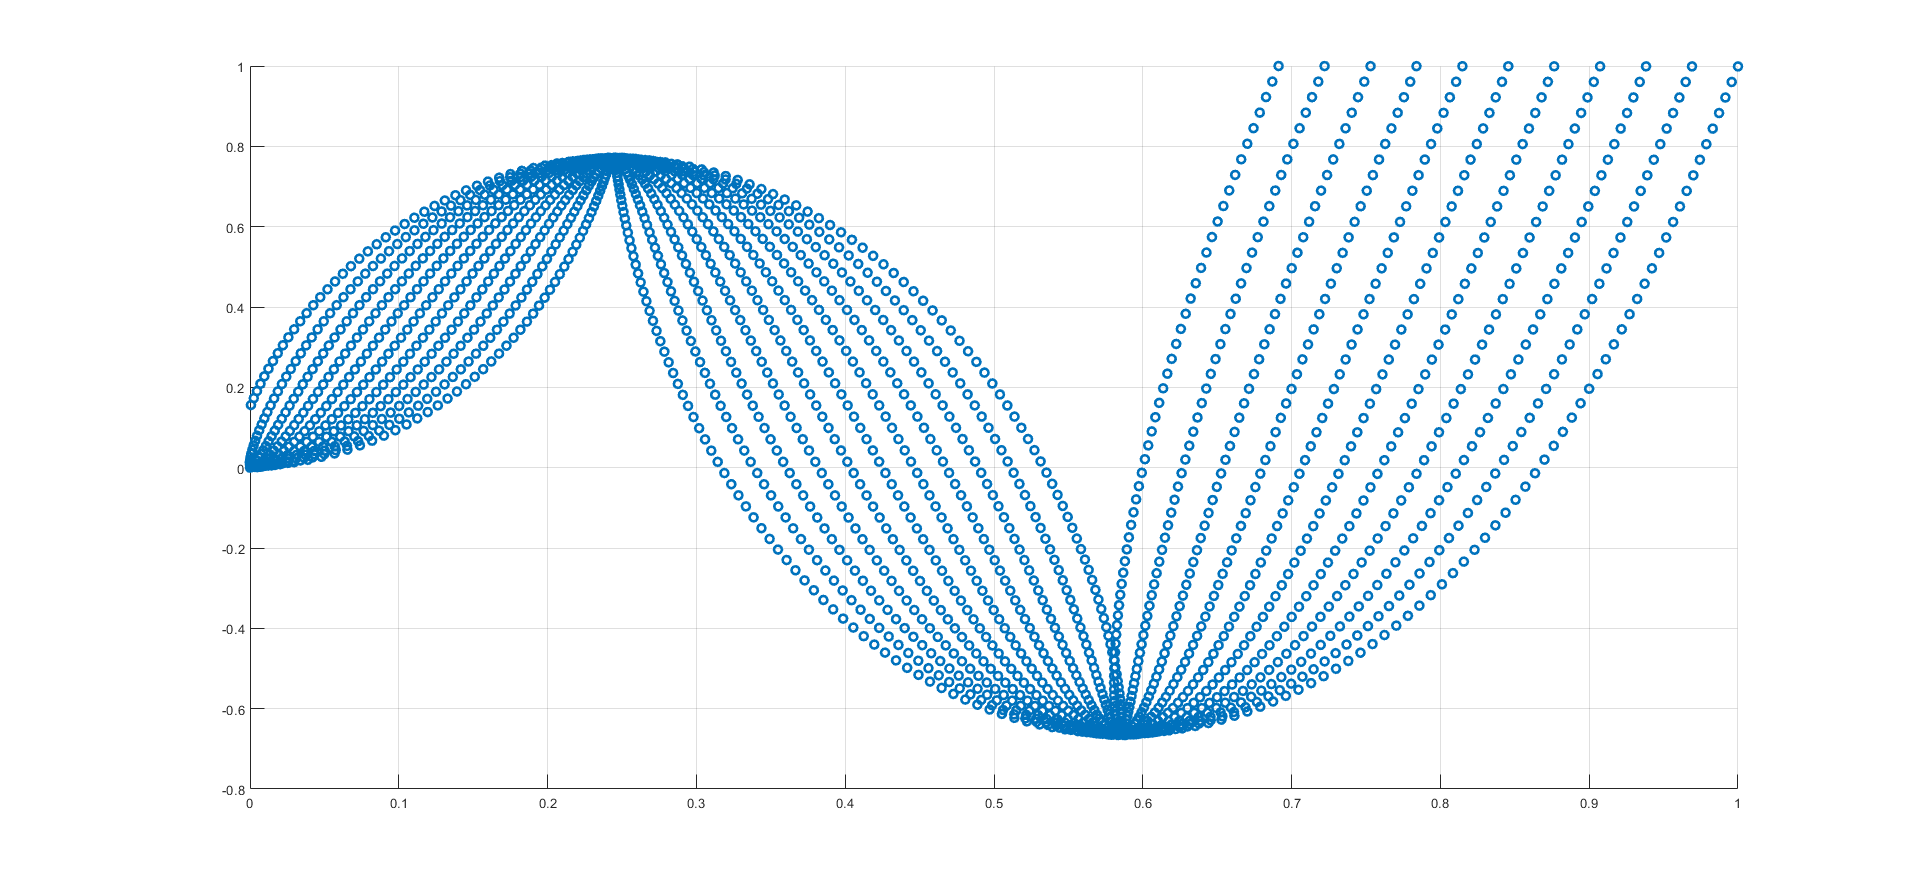
\includegraphics[width=\textwidth]{3D12.png}
                \\ 3D Beam Type - $\lambda_{12} = 2.3293$
                \label{fig:minipage2}
            \end{minipage}
            \hfill
            \begin{minipage}[b]{0.45\textwidth}
                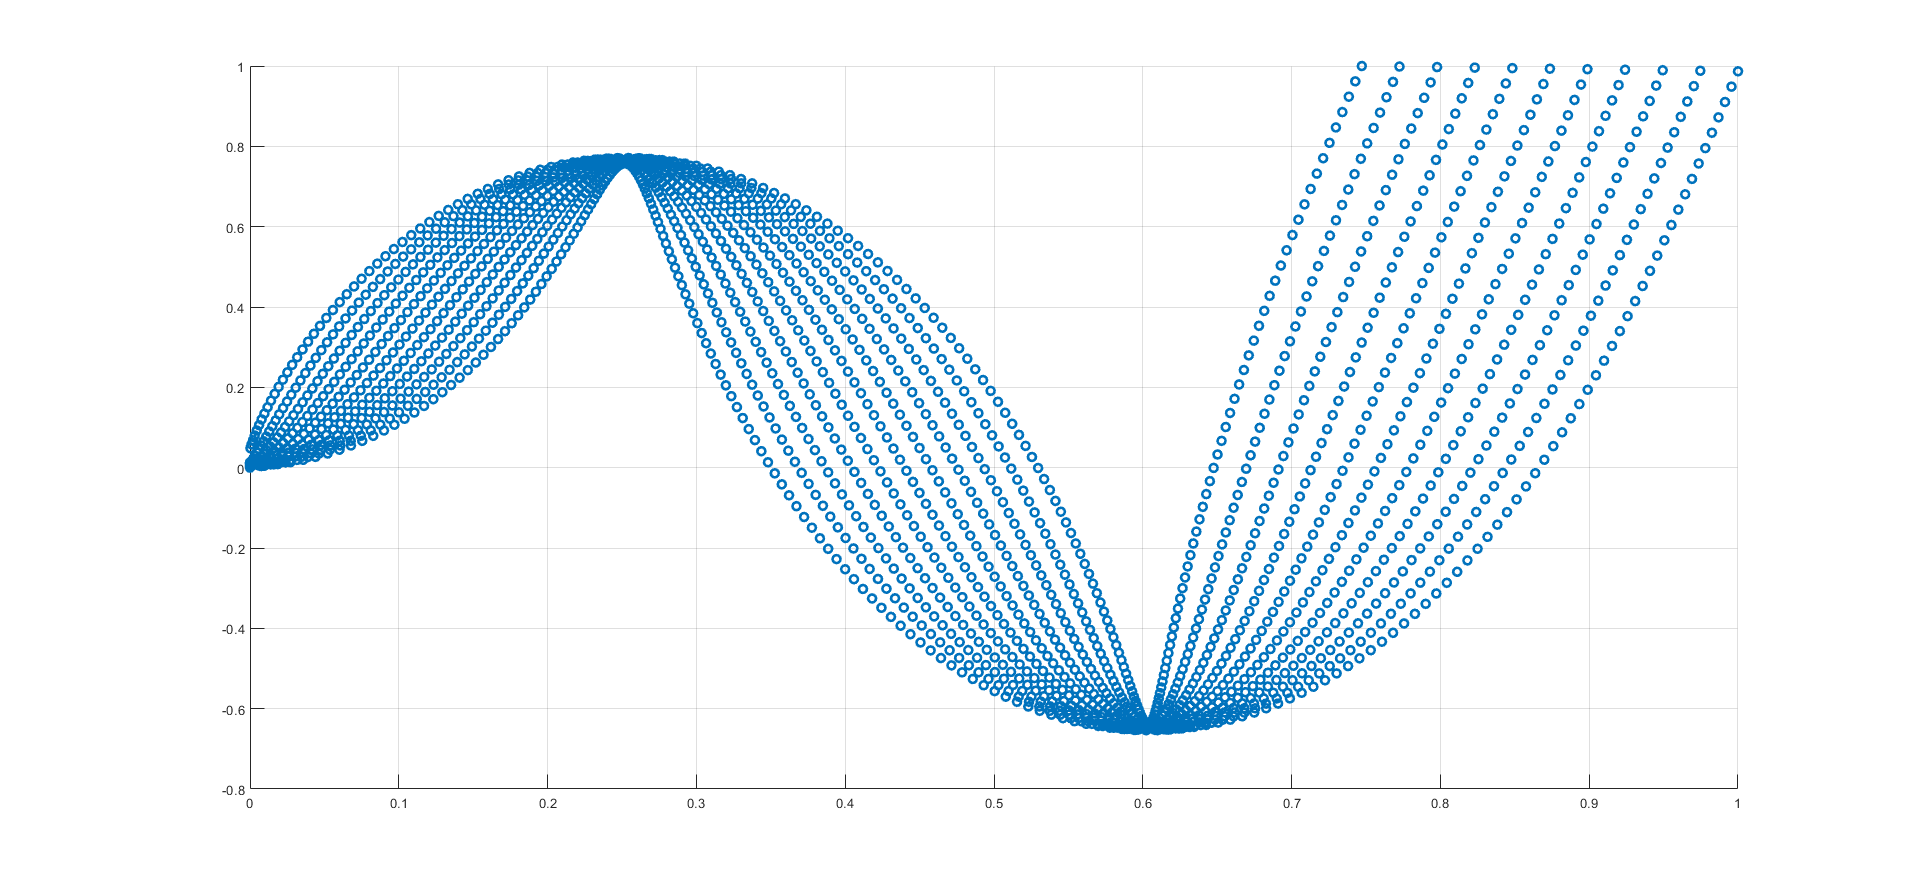
\includegraphics[width=\textwidth]{2D3.png}
                \\ 2D Beam Type - $\lambda_3 = 2.3273$
                \label{fig:minipage1}
            \end{minipage}
        
            \vspace{1em} % spacing between the rows
        
            \begin{minipage}[b]{0.45\textwidth}
                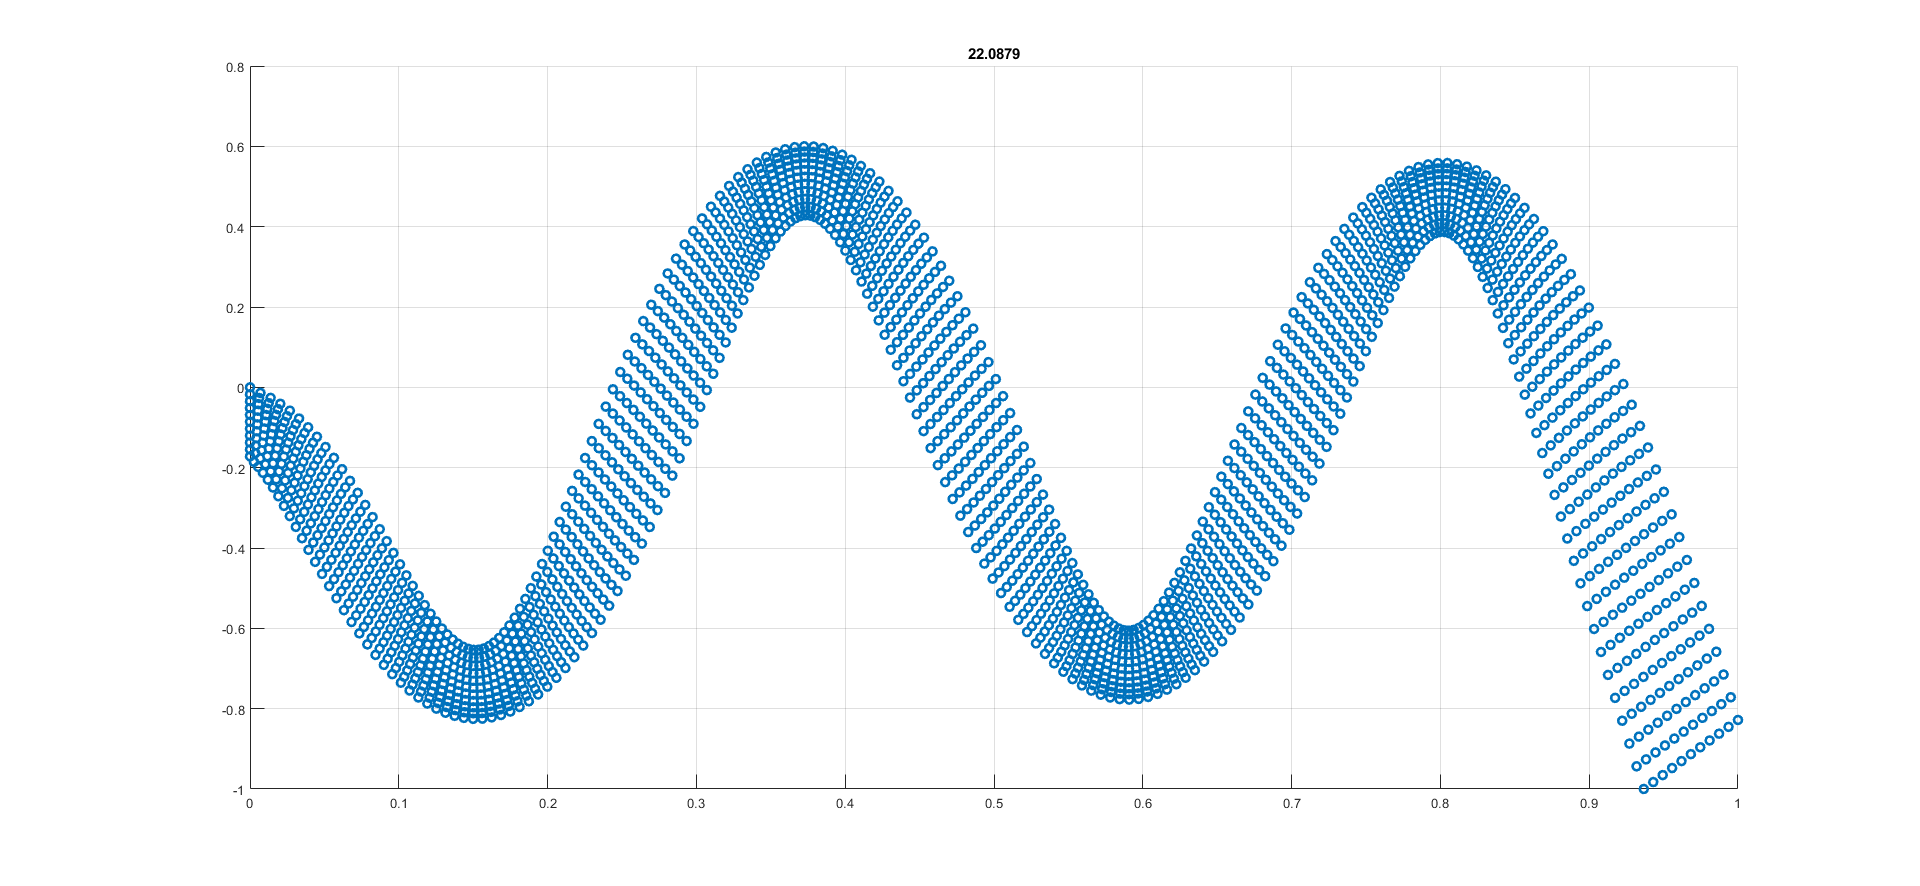
\includegraphics[width=\textwidth]{3D22.png}
                \\ 3D Beam Type - $\lambda_{24} = 21.929$
                \label{fig:minipage4}
            \end{minipage}
            \hfill
            \begin{minipage}[b]{0.45\textwidth}
                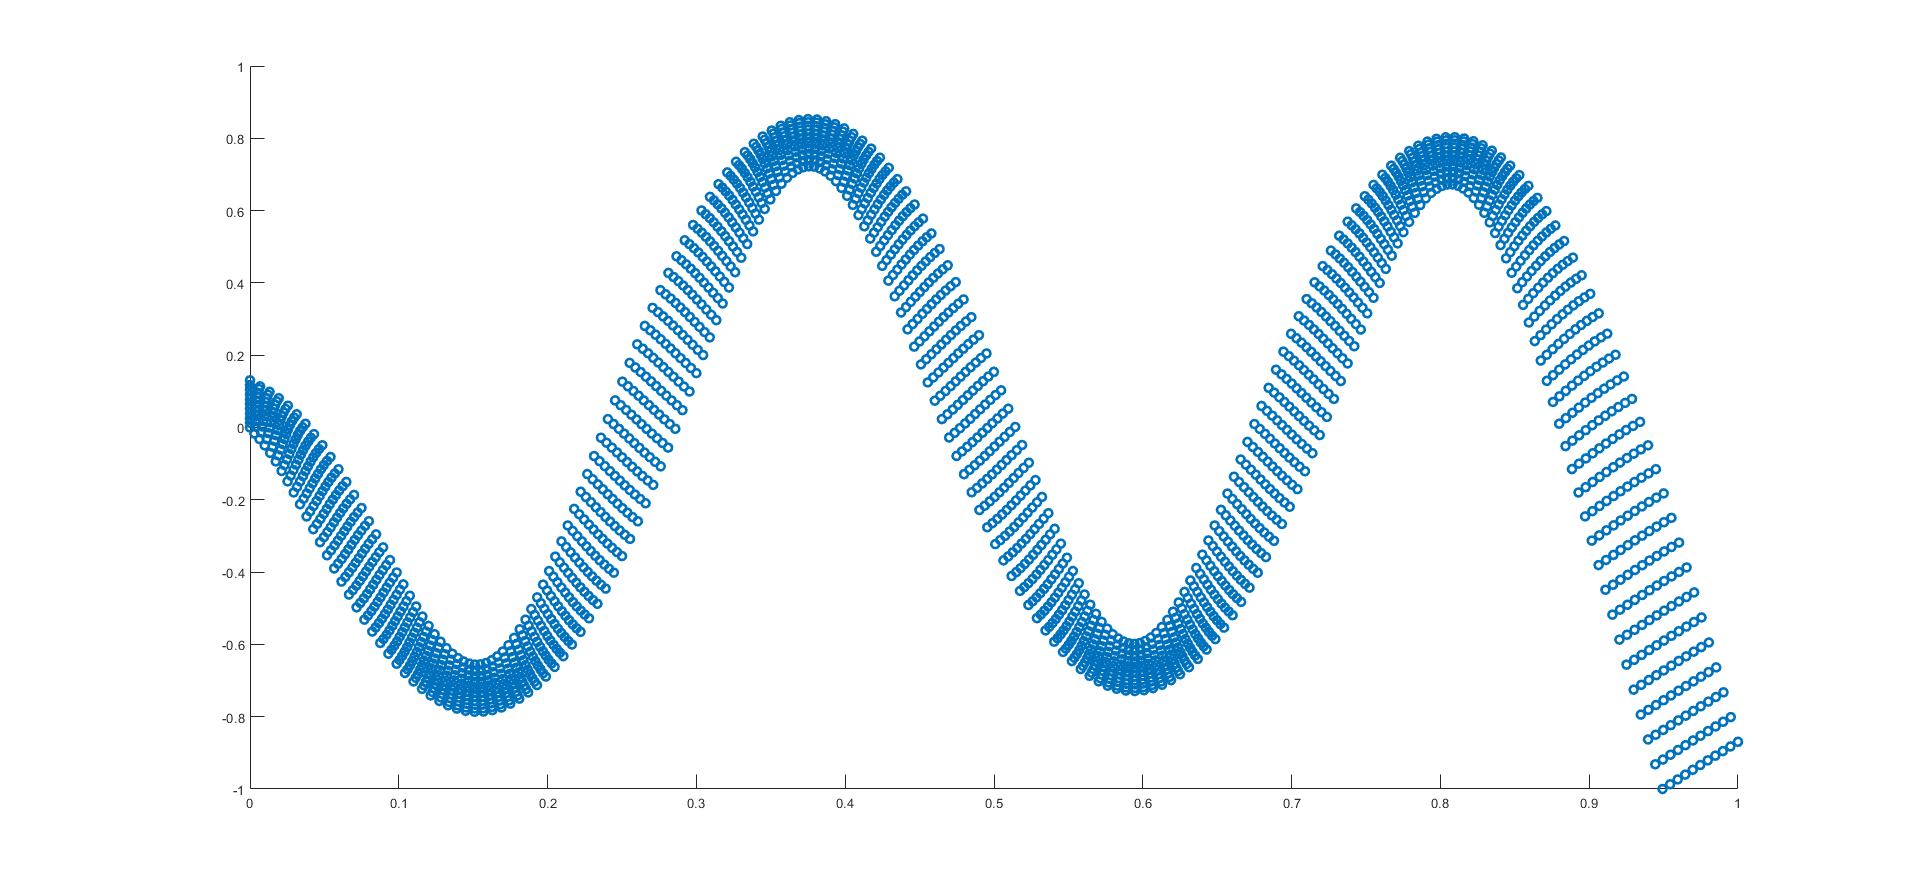
\includegraphics[width=\textwidth]{2D6.png}
                \\ 2D Beam Type - $\lambda_6 = 21.911$
                \label{fig:minipage3}
            \end{minipage}
        
            Mode shapes of the displacement \( w \) with \( h=1/20 \).
        
        \end{frame}
        
        \begin{frame}{Three-Dimensional model}
            \centering
            \begin{minipage}[b]{0.45\textwidth}
                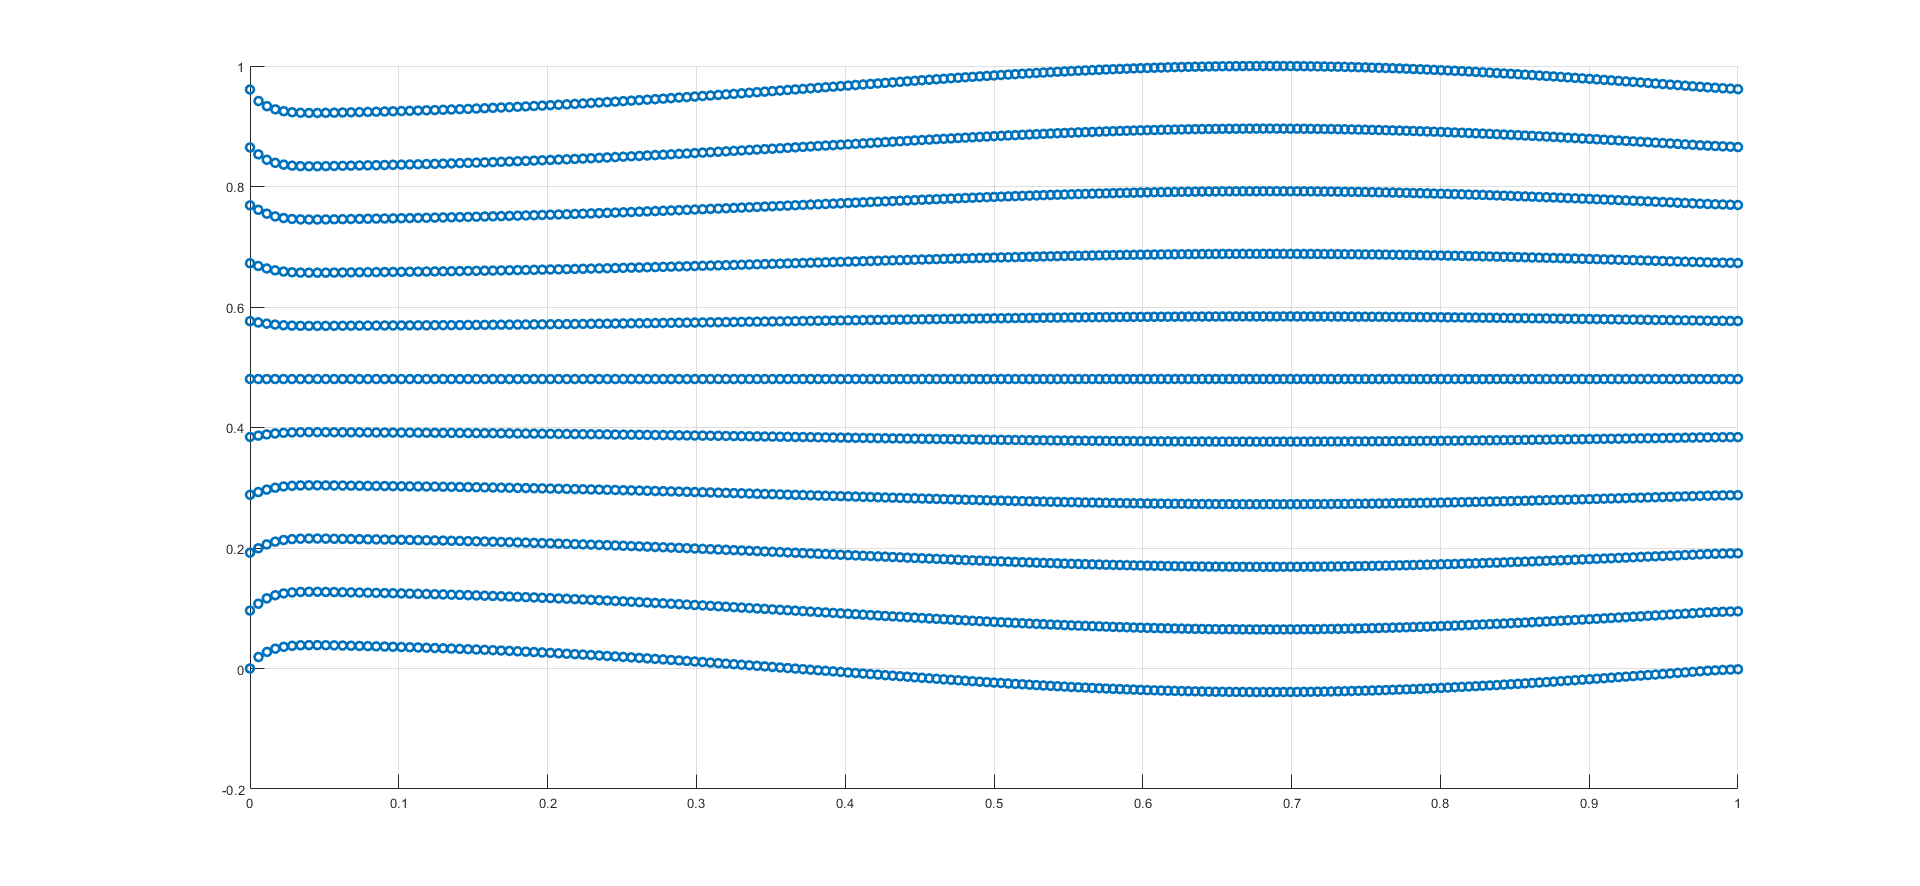
\includegraphics[width=\textwidth]{3D33.png}
                \\ 3D Non-Beam Type - $\lambda_{33} = 69.374$
                \label{fig:minipage6}
            \end{minipage}
            \hfill
            \begin{minipage}[b]{0.45\textwidth}
                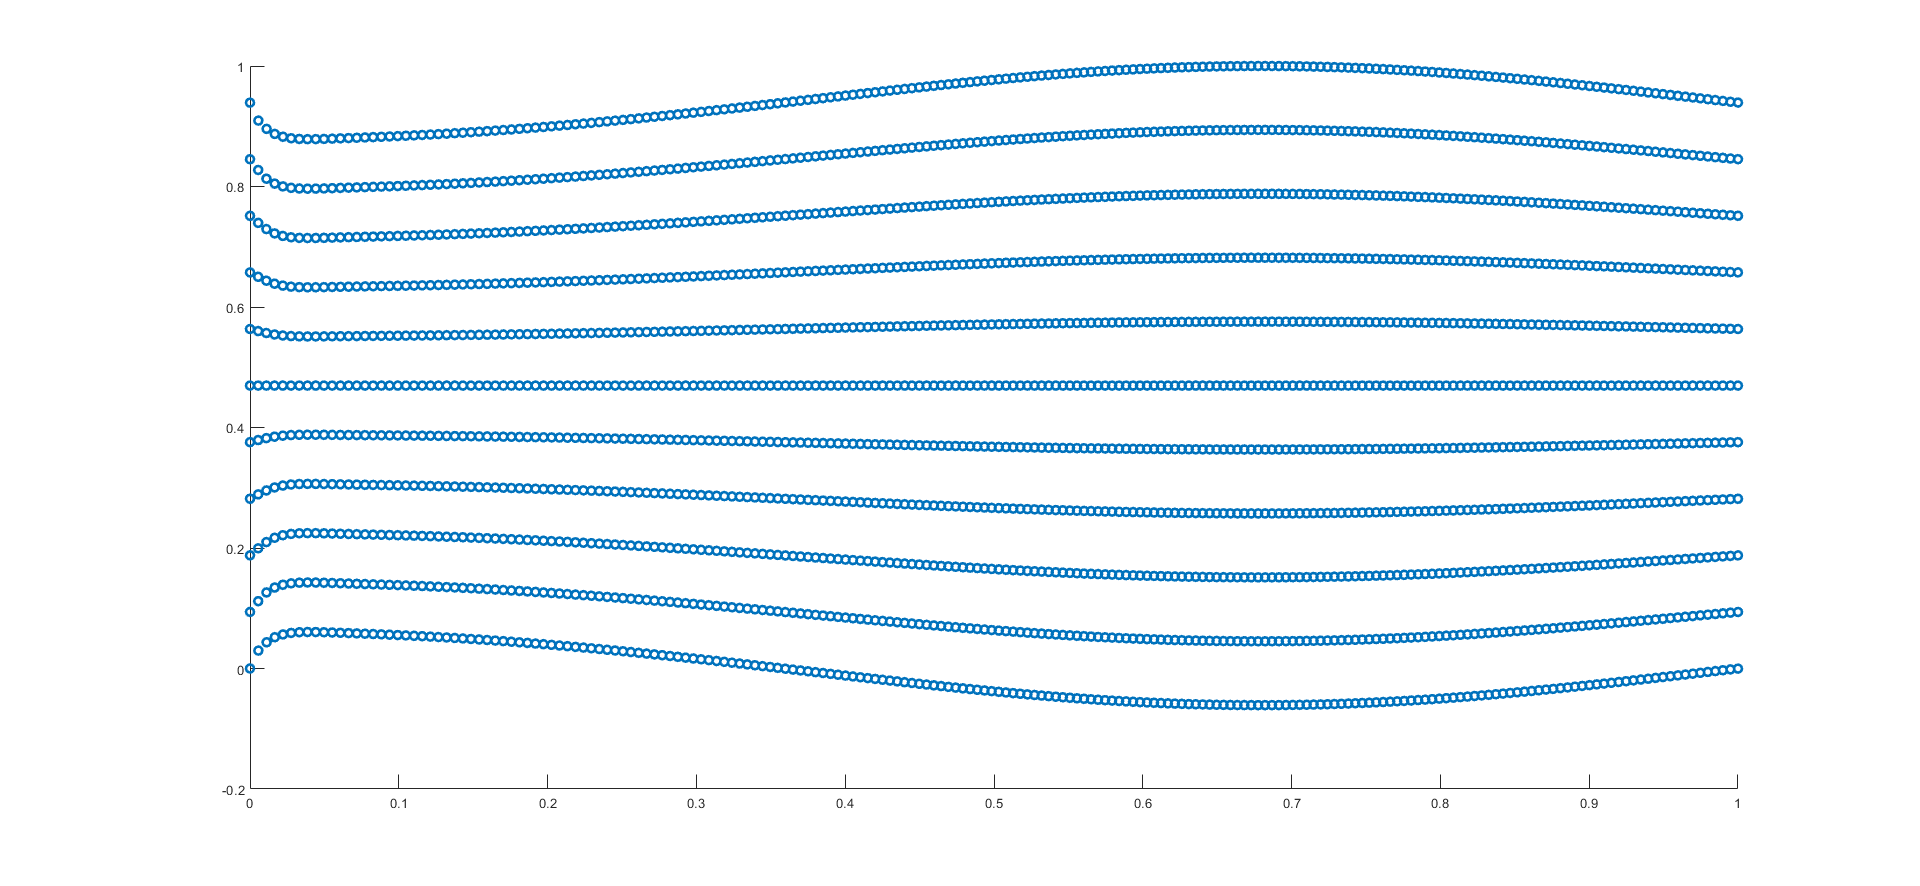
\includegraphics[width=\textwidth]{2D8.png}
                \\ 2D Non-Beam Type - $\lambda_8 = 69.344$
                \label{fig:minipage5}
            \end{minipage}
        
            \vspace{1em} % spacing between the rows
        
            \begin{minipage}[b]{0.45\textwidth}
                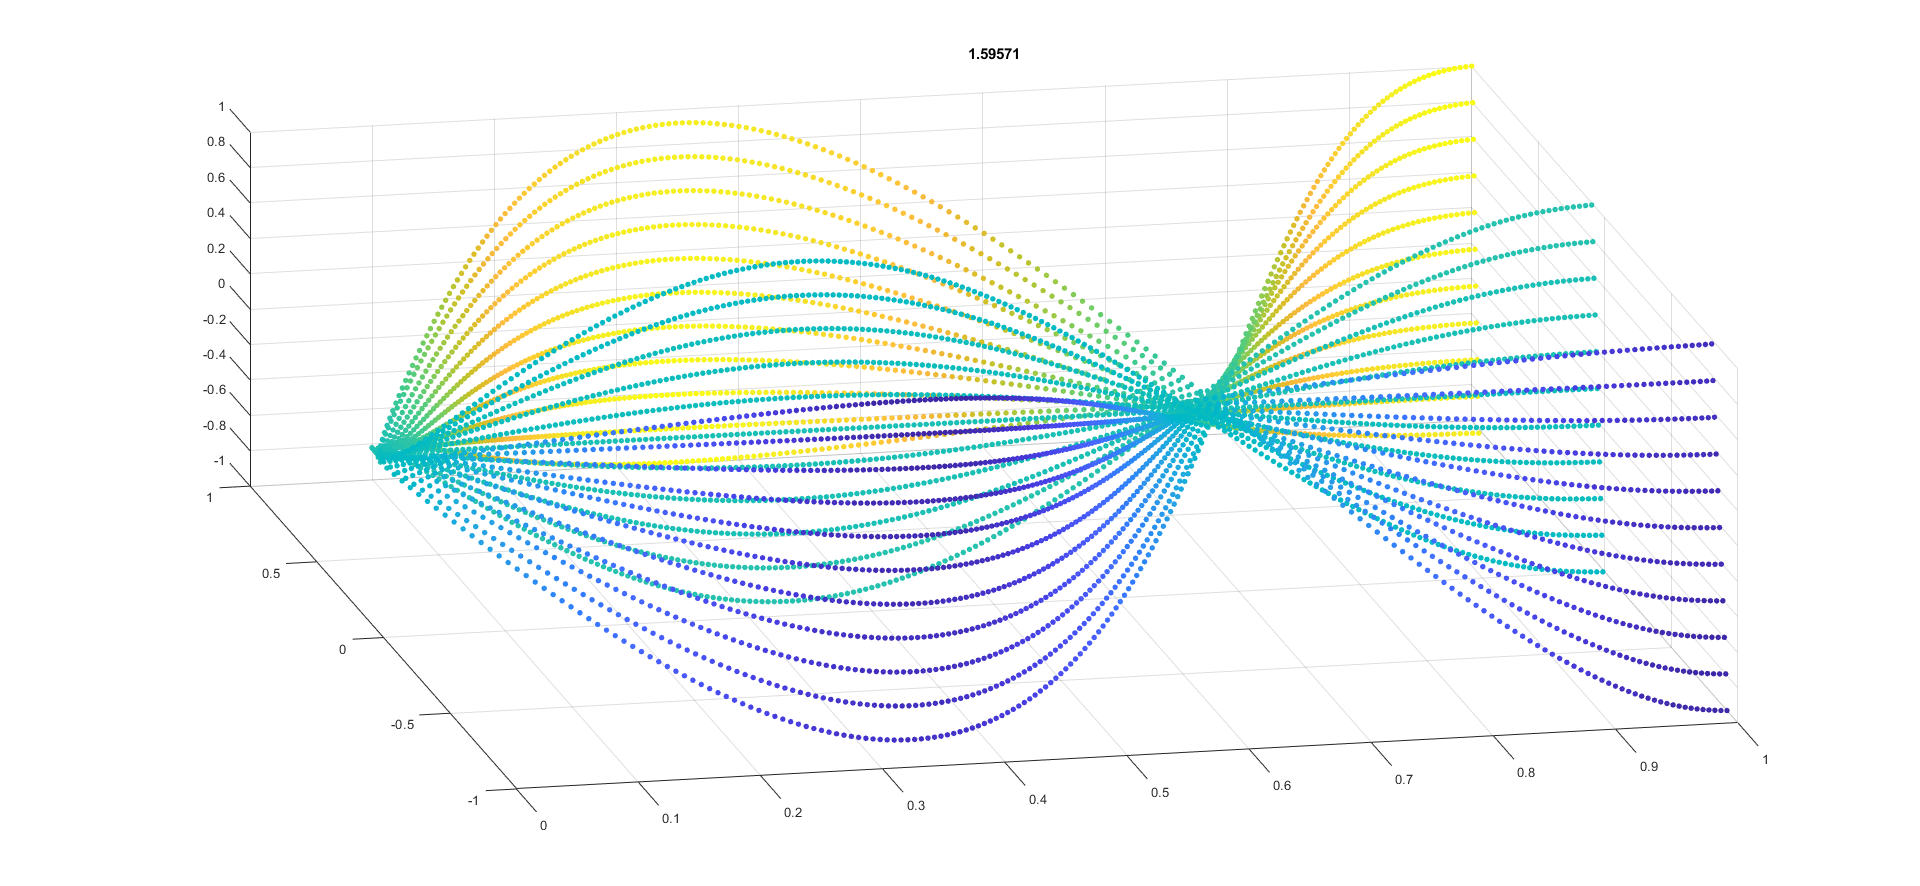
\includegraphics[width=\textwidth]{3DNonBeam10.png}
                \\ Non-2D Type - $\lambda_{10}$
                \label{fig:minipage8}
            \end{minipage}
            \hfill
            \begin{minipage}[b]{0.45\textwidth}
                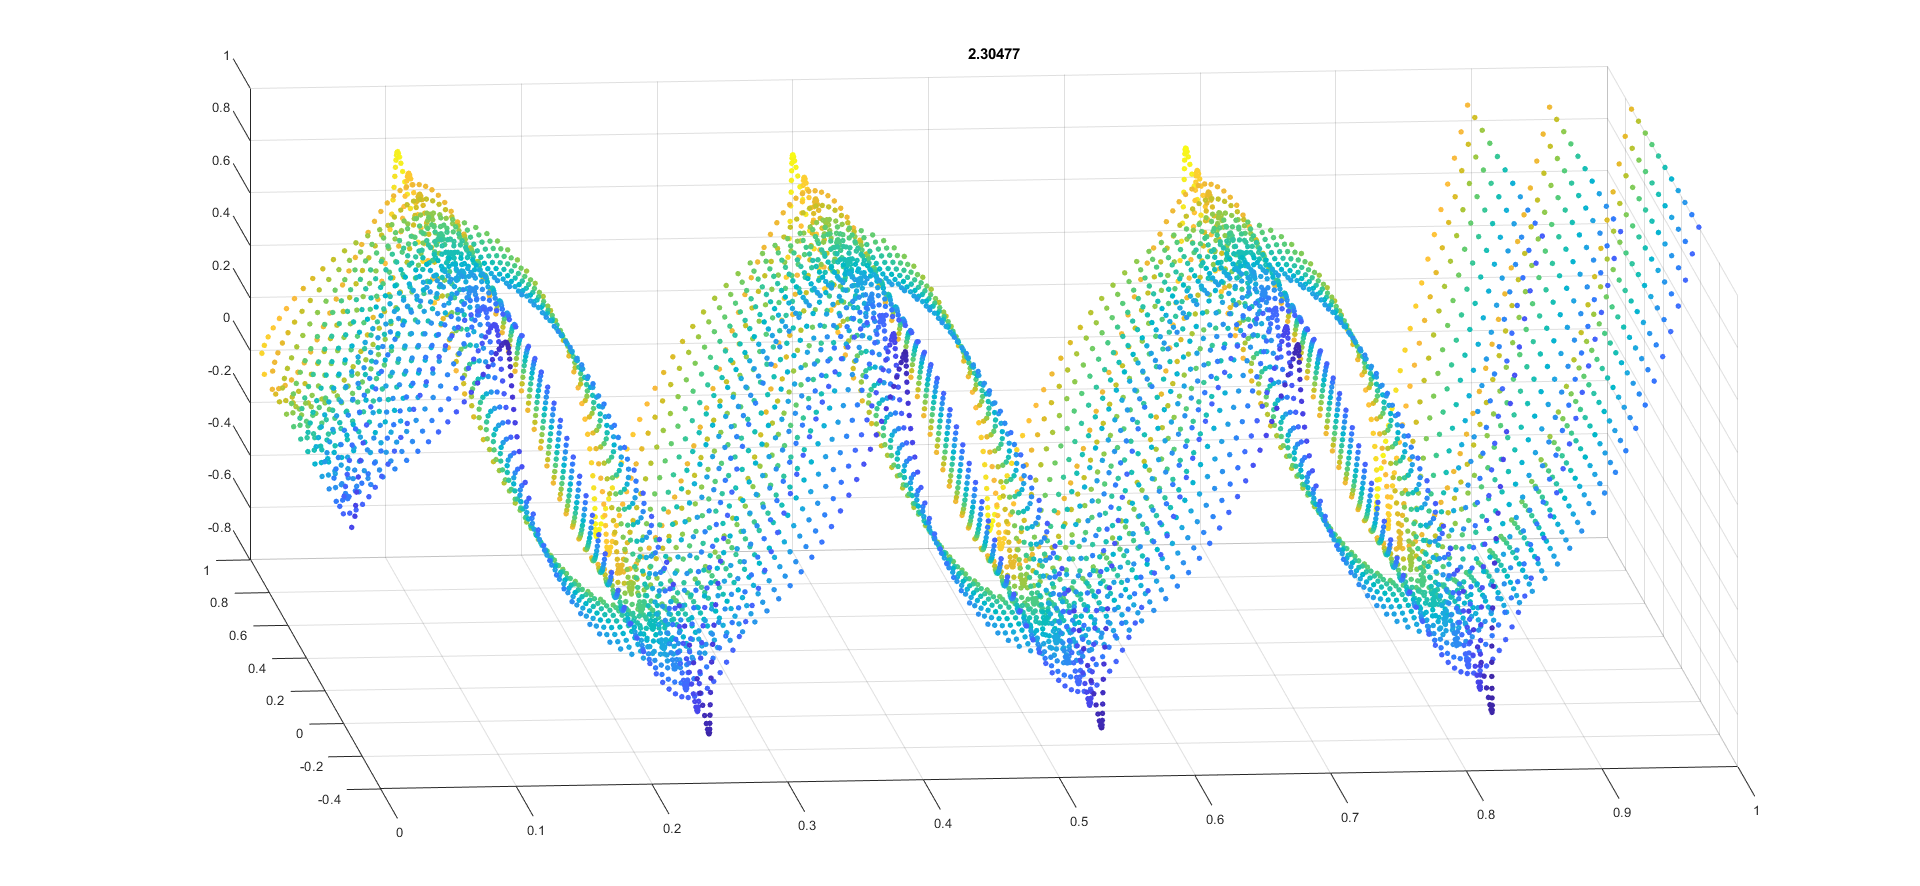
\includegraphics[width=\textwidth]{3DNonBeam11.png}
                \\ Non-2D Type - $\lambda_{11}$
                \label{fig:minipage7}
            \end{minipage}
        
            Mode shapes of the displacement \( w \) with \( \alpha = 4800 \).
        \end{frame}

\section{Conclusion}
    \begin{frame}{Conclusion}
    \end{frame}

    \begin{frame}{References}
        \printbibliography[heading=bibintoc, title={References}]
    \end{frame}

\end{document}
